\documentclass{article}
\usepackage[utf8]{inputenc}
\usepackage[T1]{fontenc} % Output font encoding for international characters
\usepackage{graphicx} % Required for including images
\usepackage{booktabs} % Required for better horizontal rules in tables
\usepackage{listings} % Required for insertion of code
\usepackage{enumerate} % To modify the enumerate environment
\usepackage{biblatex} %Imports biblatex package
\usepackage{notoccite} %Fix citation order
\addbibresource{FOV_Visualizer.bib} %Import the bibliography file
\usepackage{hyperref}
\usepackage{subcaption} % for captions for multiple images per figure
\usepackage[export]{adjustbox} %allows addition of alignment keys to \includegraphics
\usepackage{algorithm}
\usepackage{algorithmic}
\usepackage{amsmath}
\usepackage{array}



\title{	
	\normalfont\normalsize
	\textsc{National Technical University of Athens}\\ % Your university, school and/or department name(s)
	\vspace{25pt} % Whitespace
	\rule{\linewidth}{0.5pt}\\ % Thin top horizontal rule
	\vspace{20pt} % Whitespace
	{\LARGE Three Dimensional Field Of View Visualisation}\\ % The assignment title
	\vspace{5pt}
	{\LARGE Using Unity}\\
	\vspace{12pt} % Whitespace
	\rule{\linewidth}{2pt}\\ % Thick bottom horizontal rule
	\vspace{12pt} % Whitespace
}
\author{\LARGE Zarras Ioannis} % Your name
\medskip
\date{Department of Mechanical Engineering --- \today}



\begin{document}
\maketitle
\tableofcontents

\section{Overview}

The process of designing a perception system for a robot involves deciding what sensors are going to be used and what their position and rotation on the robot will be. The ability to visualise the combined field of view produced by camera and lidar sensors on the robot in simulation assists with such design decisions. There are several field of view visualisation tools freely available online but none of them is detailed, realistic or versatile enough to effectively compare multiple perception system designs in 3D space. Therefore, the goal of this project is to develop a three dimensional field of view visualisation tool and then use it to compare multiple perception system designs and reach a final decision on the design that will be used on our quadruped robot.

\section{Unity}

The Unity Development Platform was used to create the 3D simulated environment and code the behaviour of the agents in it. Unity was chosen over other simulators for several reasons:

\begin{itemize}
    \item Unity currently supports over 25 different platforms making it a highly cross-platform engine. \cite{software_what_nodate}
    \item As of 2020, Unity-made applications were used by 2 billion monthly active users, with 1.5 million monthly creators. \cite{noauthor_unity_2022}   The vast community behind Unity enables developers to ask questions and quickly find solutions to their issues.
    \item Unity is lately transitioning to Robotics, AI and simulation applications with new and actively supported packages.
\end{itemize}

\section{Usage}

\subsection{The Scene}

After downloading (from the respective Bitbucket repository) \cite{noauthor_csl_legged_nodate}, installing and launching the Unity Project, a scene that resembles a vineyard appears (Figure 1). By default, the laelaps robot model will be active in the center of the scene. On either side of the robot the user can see two rows of vines. Both the robot and the vines are scaled according to their real life dimensions. The distance between the rows of vines is also close to that of a typical real life vineyard. 

To the left of the scene tab, on the Hierarchy tab, the user can see that the vines are registered as Vine Trees under the Obstacles object category. On the scene tab, within the branches of the vines, the user can observe some blue capsules. These capsules represent bunches of grapes and are registered as targets on the Hierarchy tab, as those are the objects of interest for the robot. 

\begin{figure}
	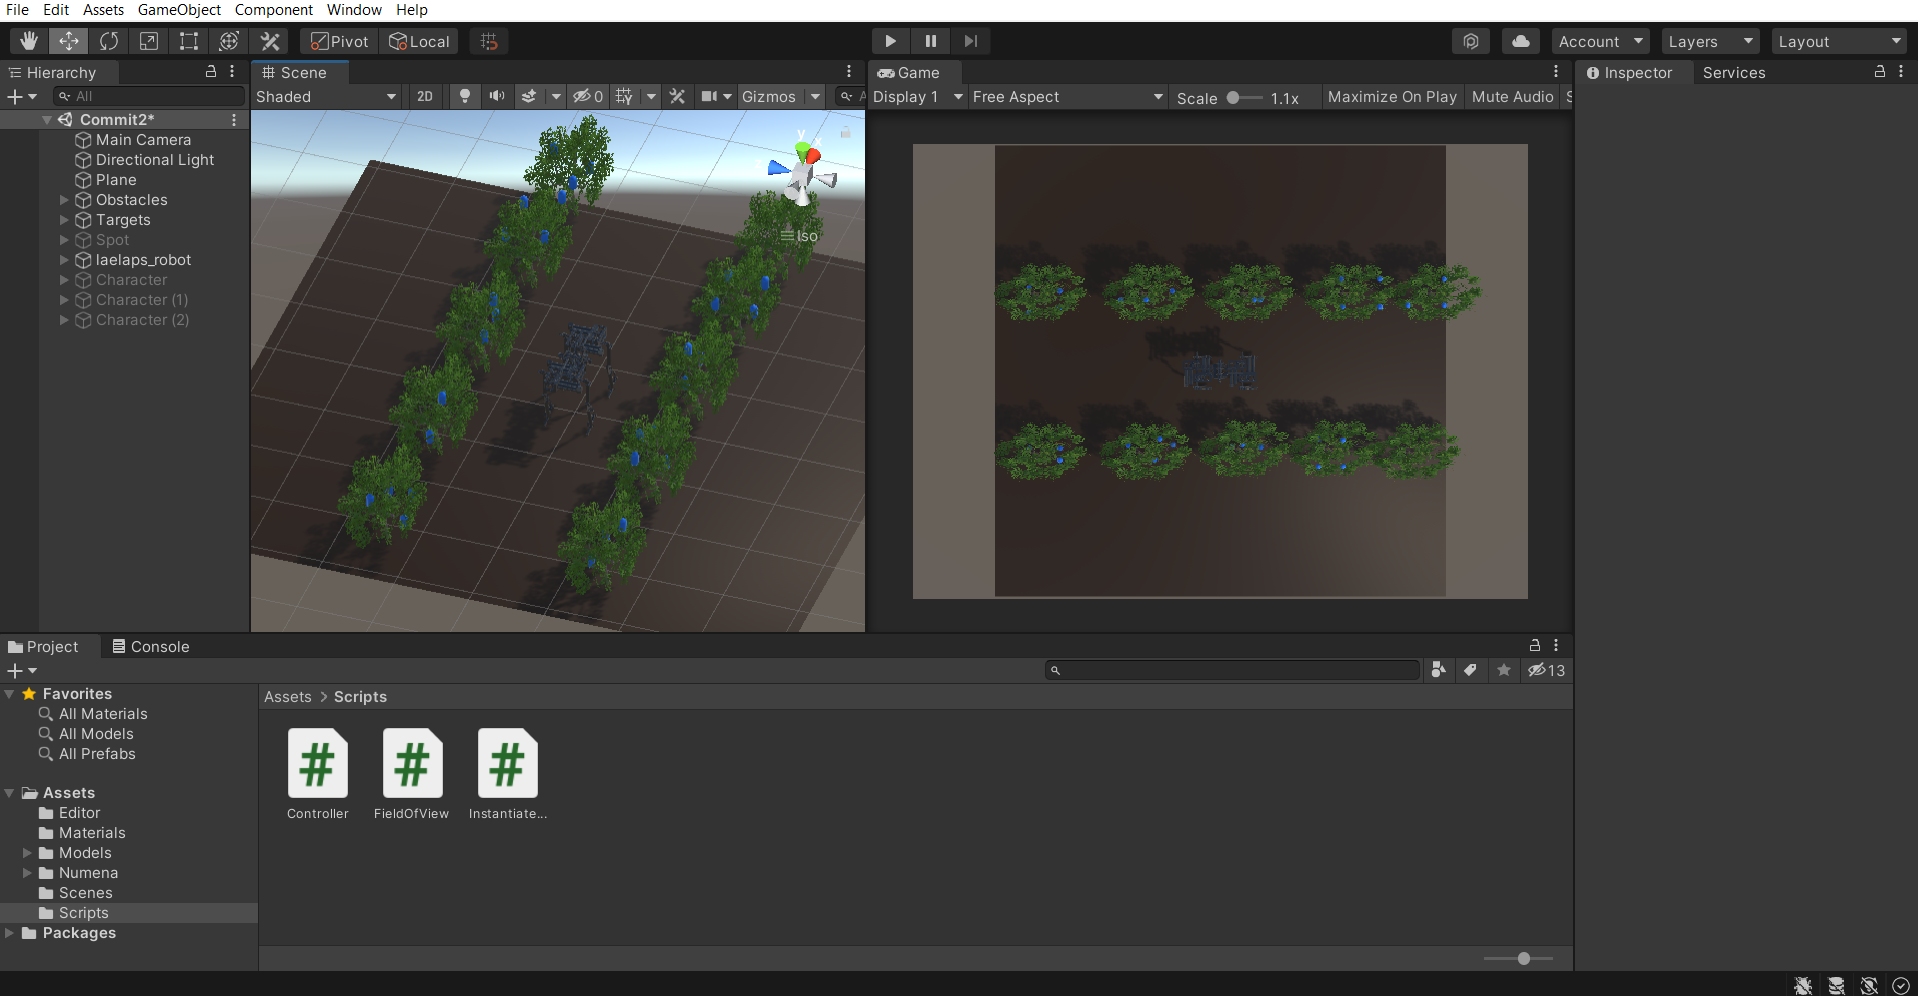
\includegraphics[width=1.7\textwidth, center]{FOV.png} % Example image
	\caption{The default starting scene in Unity.}
\end{figure}
\clearpage

In the Hierarchy tab, some object names can be seen in fainted white color. These objects are also present in the scene but they are deactivated. The user can select any of these from the Hierarchy tab. Thus, the Inspector tab on the right side of the window will display information about the selected object. To activate the selected object, the user can check the checkbox near the name of the selected object in the Inspector tab (Figure 2).

\begin{figure}[h] % [h] forces the figure to be output where it is defined in the code (it suppresses floating)
	\centering
	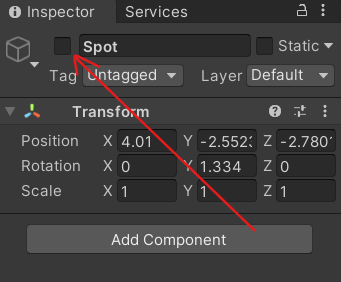
\includegraphics[width=1\columnwidth]{FOV(2).png} % Example image
	\caption{Activating and Deactivating an Object}
\end{figure}
\clearpage

The objects that are deactivated by default are the Spot robot model and three objects labeled as Sensors. The Spot robot model can be used as an alternative to the Laelaps robot model. The Sensors represent lidar (or camera) sensors and are by default placed on the sides and on the front face of the Laelaps robot model. 

Activating the three objects labeled as Sensor, Sensor (1) and Sensor (2) and clicking on play to run the simulation - the play and pause buttons are on the middle of the Unity toolbar on the top of the screen - will start the visualization of each sensor's field of view (Figure 3). 

\begin{figure}
\centering
\begin{subfigure}[b]{1\textwidth}
   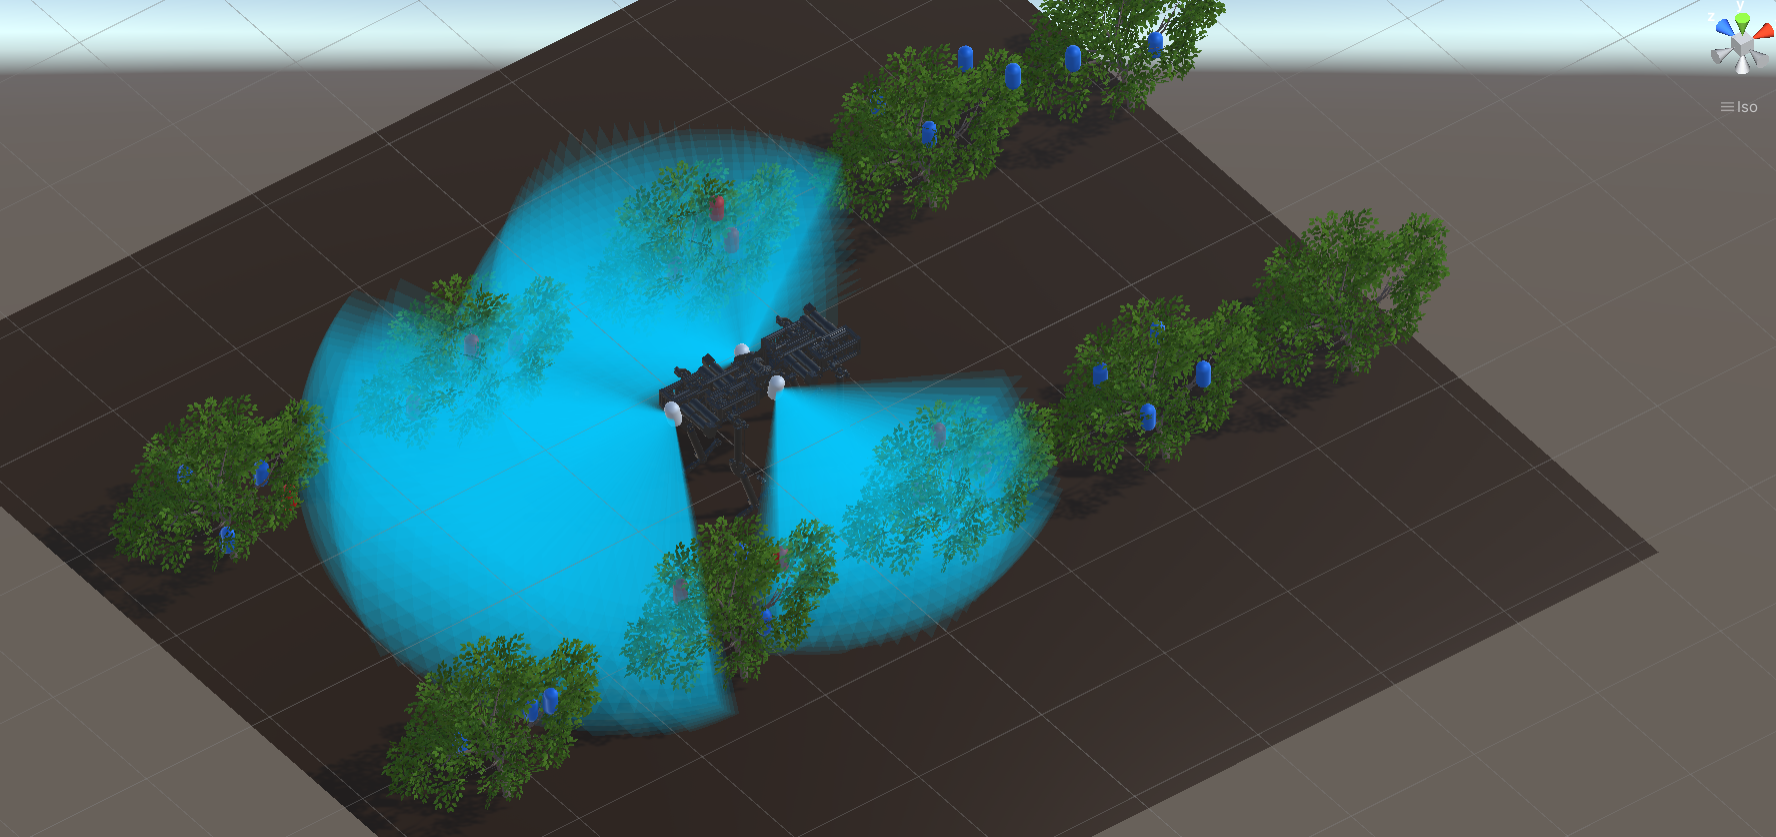
\includegraphics[width=1\linewidth]{FOV(3).png}
   \caption{Top Diagonal View}
\end{subfigure}

\begin{subfigure}[b]{1\textwidth}
   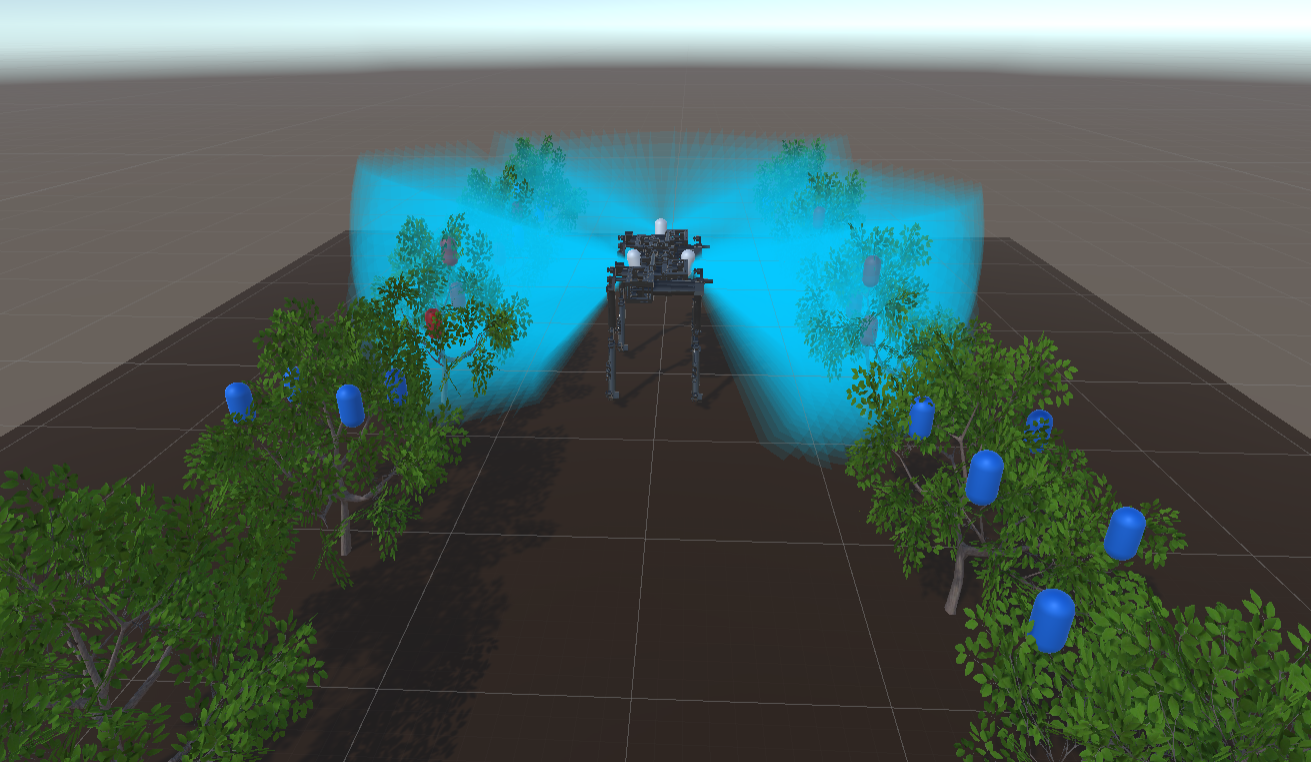
\includegraphics[width=1\linewidth]{FOV(4).png}
   \caption{Back View}
\end{subfigure}
\caption[]{The scene while running the visualization.}
\end{figure}
\clearpage

\subsection{Configuration}

The user can configure several parameters in order to simulate different sensor setups. Specifically, the list of parameters that can be configured for each sensor is as follows:

\begin{itemize}

\item position(x,y,z) : The position of the sensor in the scene, relative to the center of the scene (Which for the commit2.unity scene is also the center of the plane, as well as the center of the laelaps robot urdf). Values are in decimeters.
\item rotation(x,y,z) :  The rotation of the sensor in the scene, relative to the center of the scene (Which for the commit2.unity scene is also the center of the plane, as well as the center of the laelaps robot urdf). Values are in degrees.
\item View Radius : The range of the lidar while scanning horizontally (or max range for camera). 
\item View Angle : The horizontal view angle of the lidar (or camera).
\item Vertical View Radius : The range of the lidar while scanning vertically (or max range for camera).
\item Vertical View Angle : The vertical view angle of the lidar (or camera).
\item Mesh Resolution : Number of rays cast for each horizontal mesh divided by the horizontal view angle in degrees (See section "How it was made" for more intuition).
\item Horizontal Offset Resolution : Number of horizontal meshes to be cast, divided by the vertical view angle in degrees (See section "How it was made" for more intuition).
\item Vertical Mesh Resolution : Number of rays cast for each vertical mesh divided by vertical view angle in degrees (See section "How it was made" for more intuition).
\item Vertical Offset Resolution : Number of vertical meshes to be cast, divided by the horizontal view angle in degrees. (See section "How it was made" for more intuition). 
\item Edge Resolve Iterations : Binary search iterations to resolve the "edge problem" (See section "How it was made" for more intuition). 
\item Edge Distance Threshold : Minimum distance at which an obstacle would be considered to be too far to be accounted for the resolution of the "edge problem" (See section "How it was made" for more intuition). 

\end{itemize}

There are two ways to easily set the position and rotation of the sensors on the scene as well as to configure the sensor parameters: One is through modifying the instantiation.txt file located in the project folder. The other is using the Unity Editor to directly edit the scene and the sensor parameters.

\subsubsection{Configuration using the instantiation file}

The "instantiation.txt" file is located inside the project folder. Essentially, the instantiation file represents an array. The elements of the array inside each row are separated by commas as the file is in csv format. The first row contains the headers of each column. Each row added after the first will cause the instantiation of a new sensor on the scene. The new sensor's parameters will be the elements of the new row in correspondence with the headers. As an example, the "typical\_instantiation.txt" can be used to instantiate three sensors at the positions and rotations of the preexisting sensors  Sensor, Sensor (1) and Sensor (2) in the object hierarchy. These sensors are also parameterized identically to the preexisting sensors in the object Hierarchy. To try the instantiation file, the user can copy the contents of "typical\_instantiation.txt" inside the "instantiation.txt" file, deactivate the preexisting sensors in the scene and run the simulation. If the "instantiation.txt" file cannot be edited while the Unity Development Platform is open, then the user might need to close it when editing and then open it again to run the simulation. 


\subsubsection{Configuration using the Unity Editor}

In the unity editor, the user can activate, deactivate or duplicate the preexisting sensors Sensor, Sensor (1) and Sensor (2) which can be found in the object Hierarchy. Clicking on a sensor object triggers the inspector to show information about that object. The user can configure all the aforementioned parameters by editing the field of view script for each sensor directly in the Inspector. In this case, the "instantiation.txt" file should be empty except for the first row (except, of course, if the user desires to both have sensors preexisting in the scene and also instantiate some more sensors when starting the simulation). To change the position and rotation of the sensors on the scene, the user can use the move and rotate tools that the Unity Editor offers.

\section{How it was made}

\subsection{Forming a single horizontal mesh}
    
    It is simpler to first study how a single horizontal 2D mesh is made. Similarly to the method used in \cite{sebastian_lague_field_2015}, a number of rays is casted from the center of the sensor radially inside the horizontal view angles determined by the user, as seen in Figure 4. The number of rays for a given field of view angle is determined by the mesh resolution parameter which can be configured by the user. Rays do not pass through obstacles. The starting and ending point of each ray are sequentially saved in a list as 3D points. This list is then used with Unity's Mesh class to form a flat mesh (Figure 5). The higher the mesh resolution, the more accurate the mesh. 
    
\begin{figure} % [h] forces the figure to be output where it is defined in the code (it suppresses floating)
	\centering
	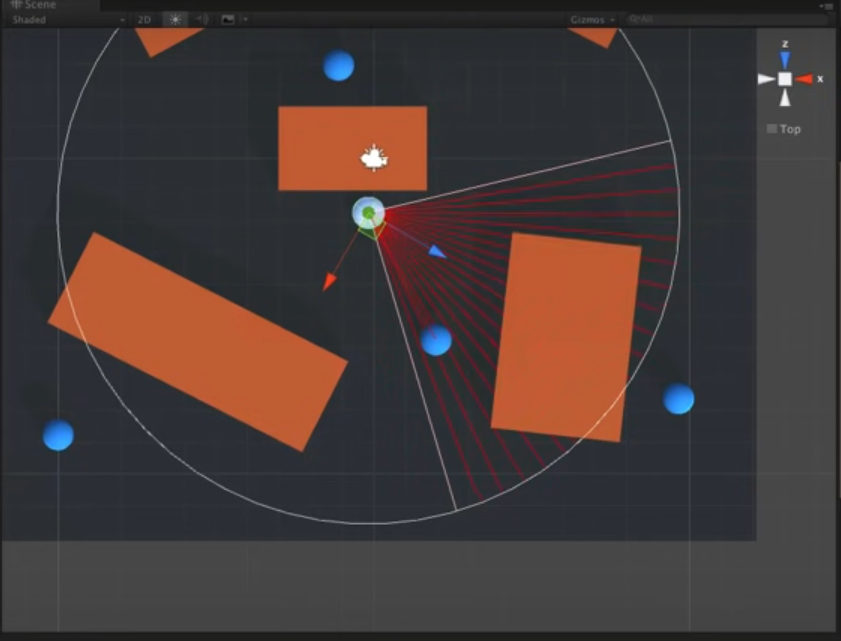
\includegraphics[width=1\columnwidth]{FOV(5).png} % Example image
	\caption{Raycasting visualization. The sensor is the white capsule. Rays are in red color. Targets are blue capsules. Obstacles are orange rectangular cuboids.}
\end{figure}

\begin{figure} % [h] forces the figure to be output where it is defined in the code (it suppresses floating)
	\centering
	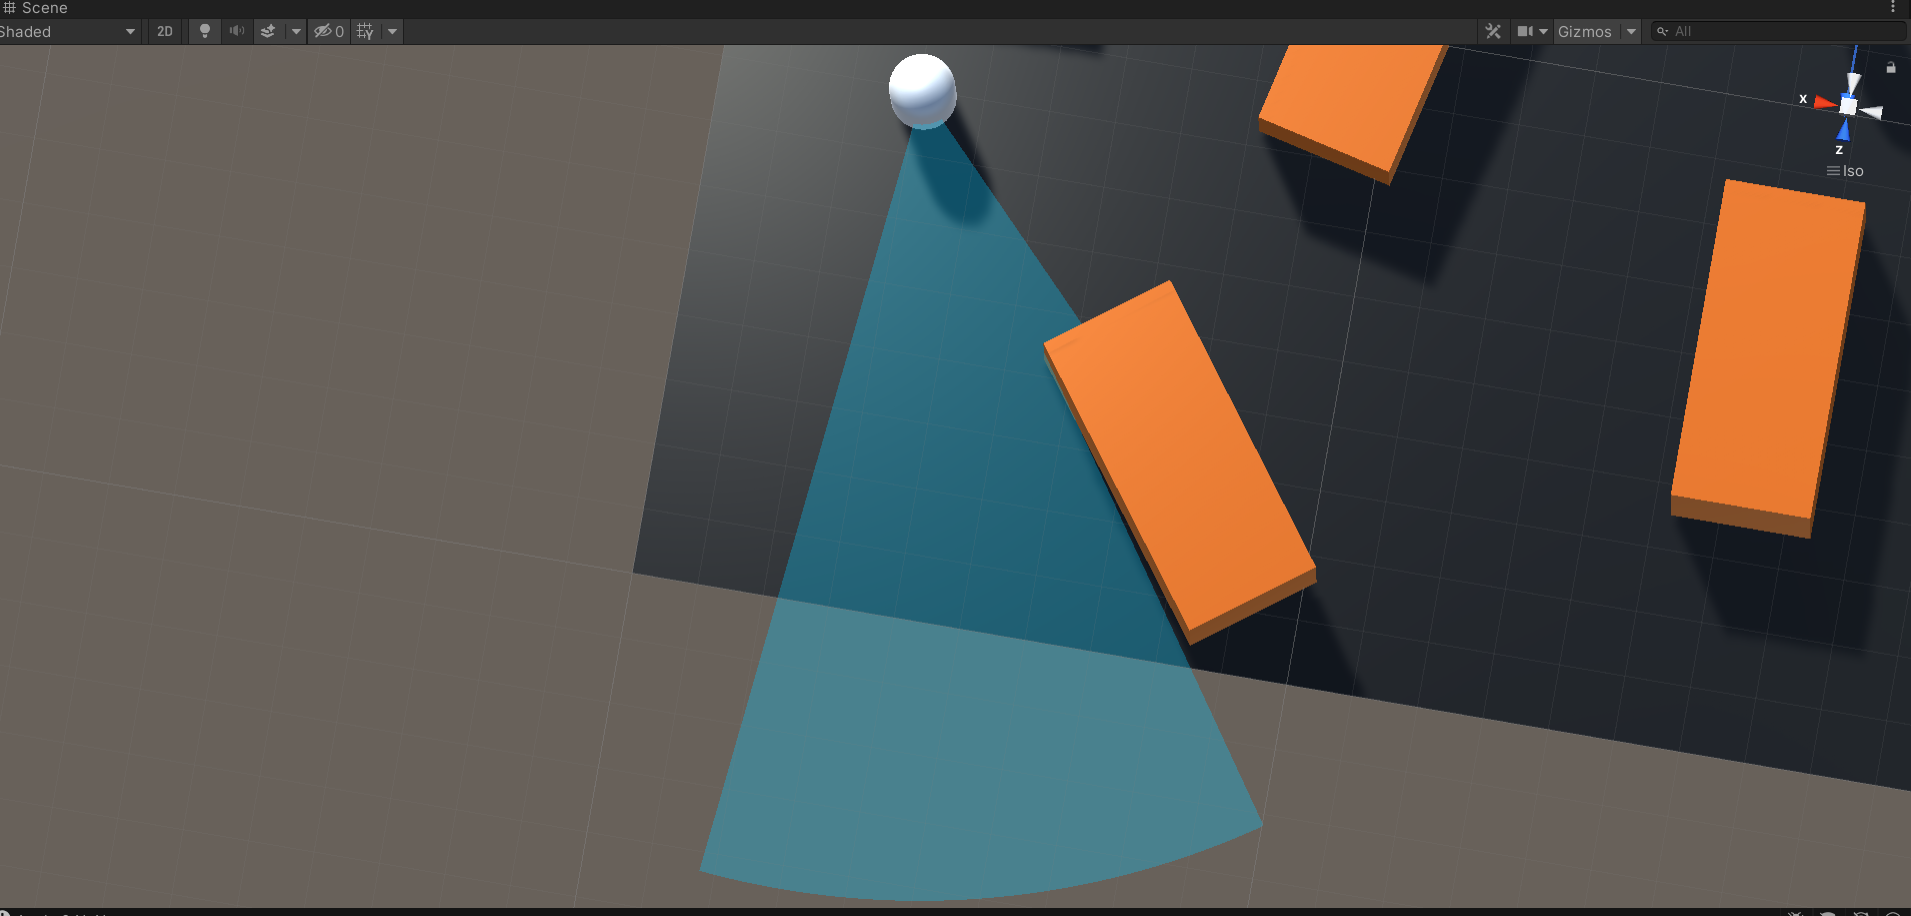
\includegraphics[width=1\columnwidth]{FOV(6).png} % Example image
	\caption{A continuous 2D mesh in light blue color.}
\end{figure}

\subsubsection{The edge problem}

The edge problem arises when the edge of an obstacle lies between any two casted rays. Thus, one ray hits an obstacle and the next one misses, ending on the view radius. The two endpoints of the rays that are used to form the mesh by the mesh renderer are now forming a triangle that passes through the obstacle. That does not represent the actual field of view correctly, as seen in Figure 6. 

\begin{figure} % [h] forces the figure to be output where it is defined in the code (it suppresses floating)
	\centering
	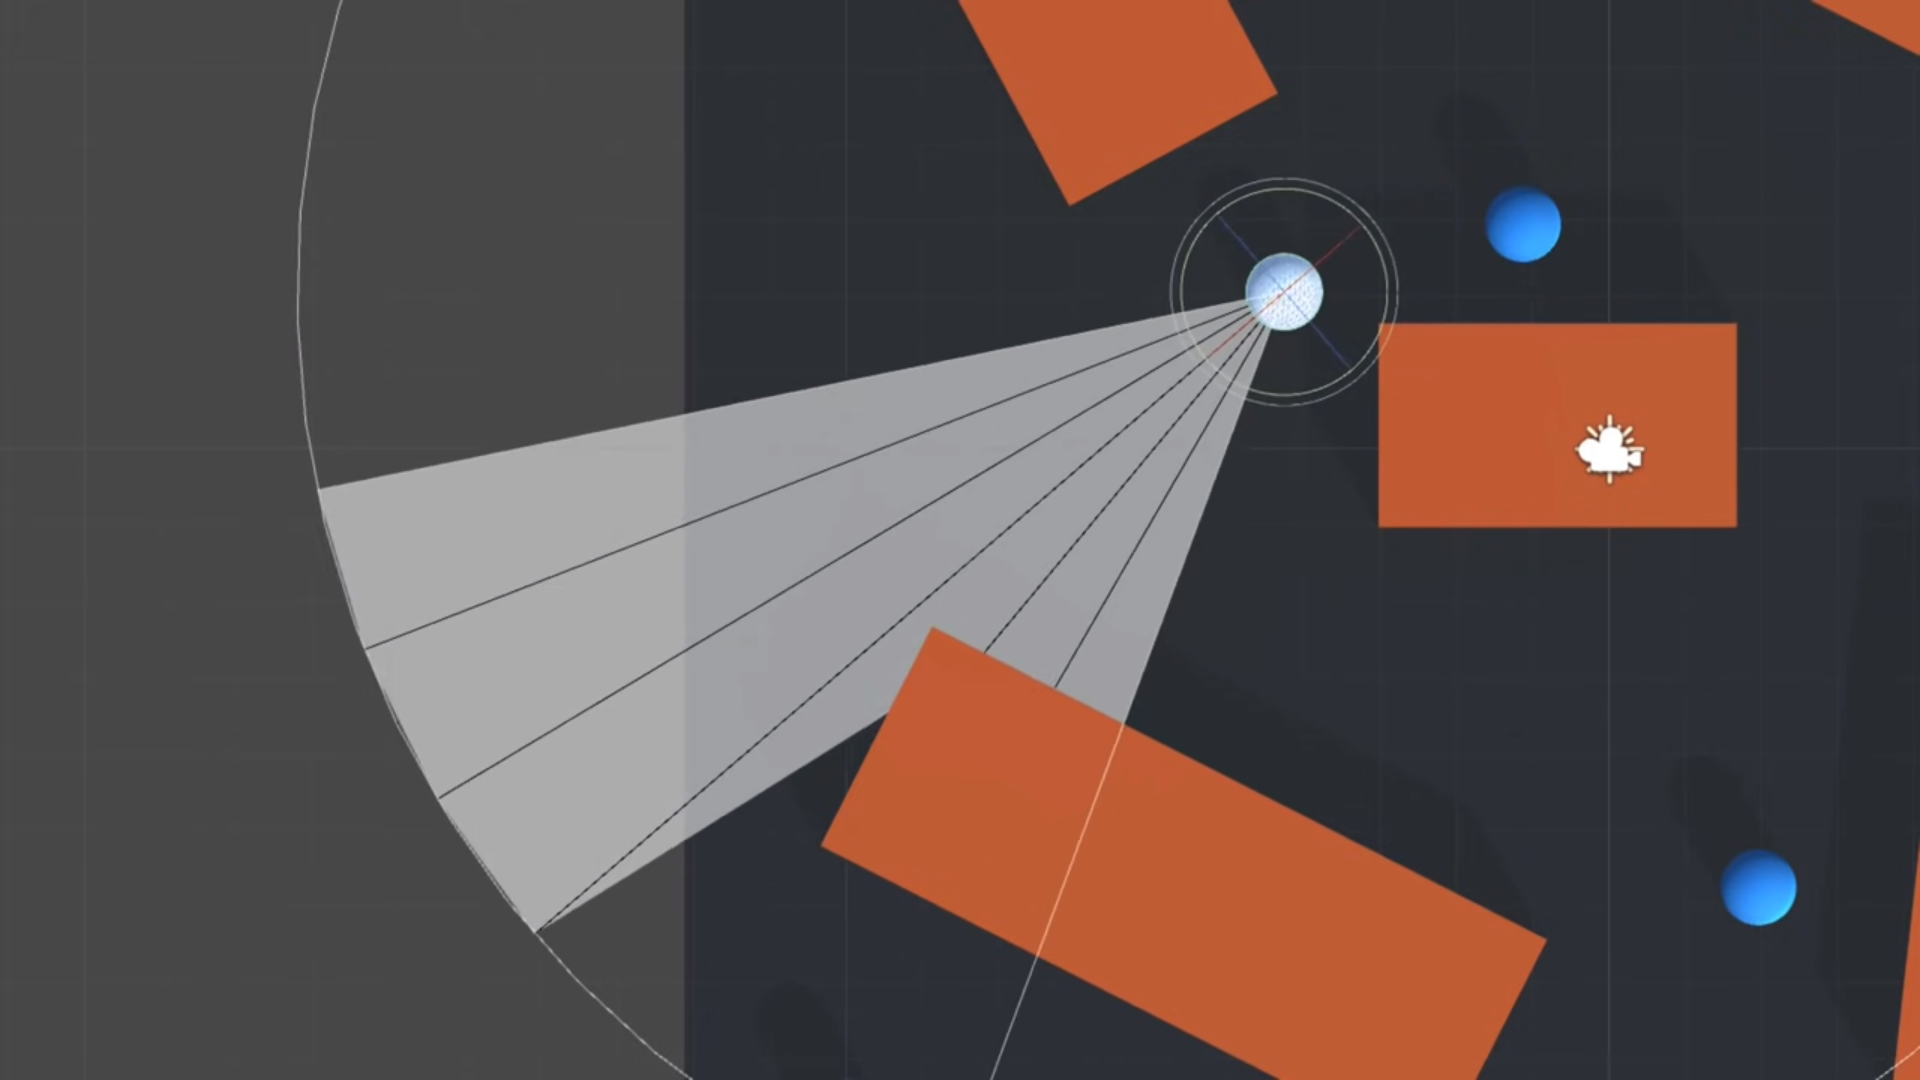
\includegraphics[width=1\columnwidth]{FOV(7).png} % Example image
	\caption{The edge problem can be clearly seen if the mesh resolution is lowered down enough.}
\end{figure}

To solve the problem, we perform a binary search of angles between the angles of said two rays, until an angle, namely a ray direction, that passes closely enough to the edge, is found. Then we cast a ray in that direction. The more the iterations of the performed binary search, the closer the new ray will be at the real edge. The number of iterations can be adjusted by the user by modifying the EdgeResolveIterations parameter. The result can be seen in Figure 7. 

\begin{figure} % [h] forces the figure to be output where it is defined in the code (it suppresses floating)
	\centering
	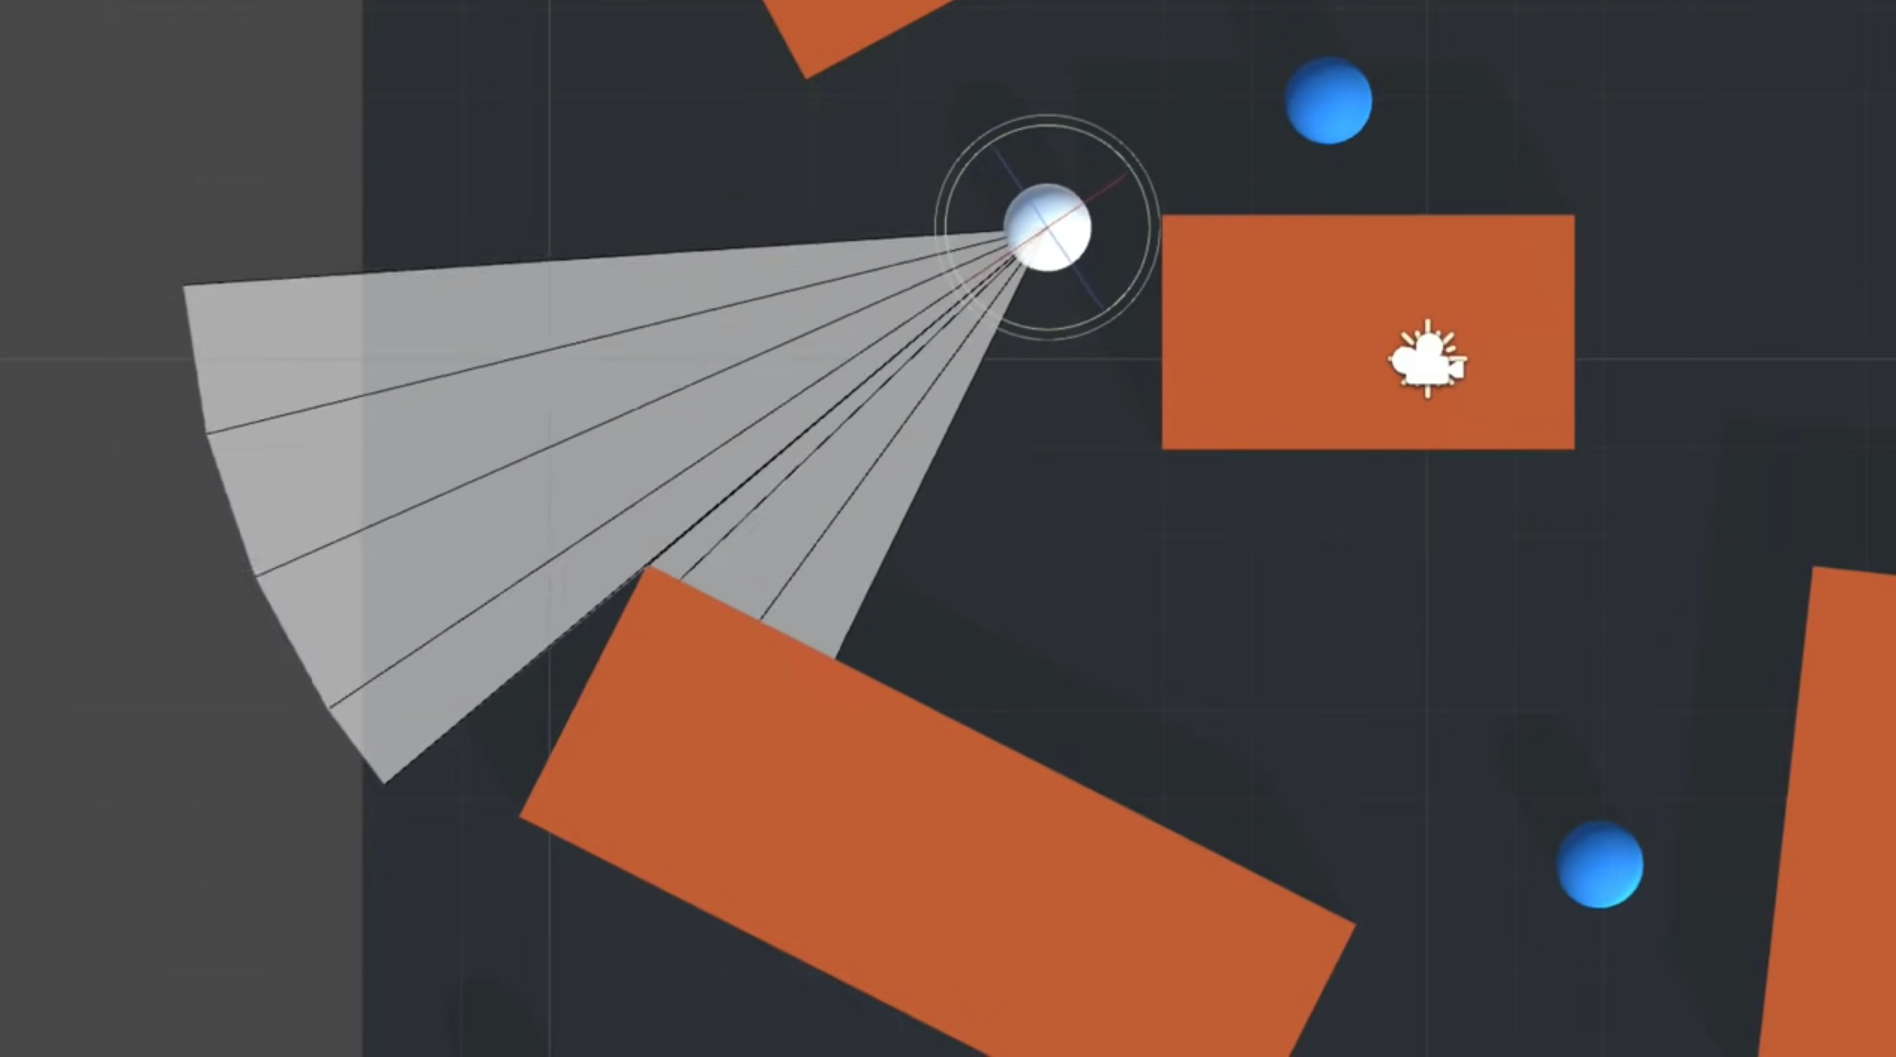
\includegraphics[width=1\columnwidth]{FOV(8).png} % Example image
	\caption{Solving the edge problem with 5 binary search iterations.}
\end{figure}

There is however a problem regarding the condition which triggers the solution of the edge problem. Currently, the condition is that when one ray hits an obstacle and the next one does not hit an obstacle, ending on the view radius, the solution of the edge problem is triggered. The problem is that when both rays hit, but the hit points are a large distance apart, the solution should be triggered, but it does not. This is shown in Figure 8. 

\begin{figure} % [h] forces the figure to be output where it is defined in the code (it suppresses floating)
	\centering
	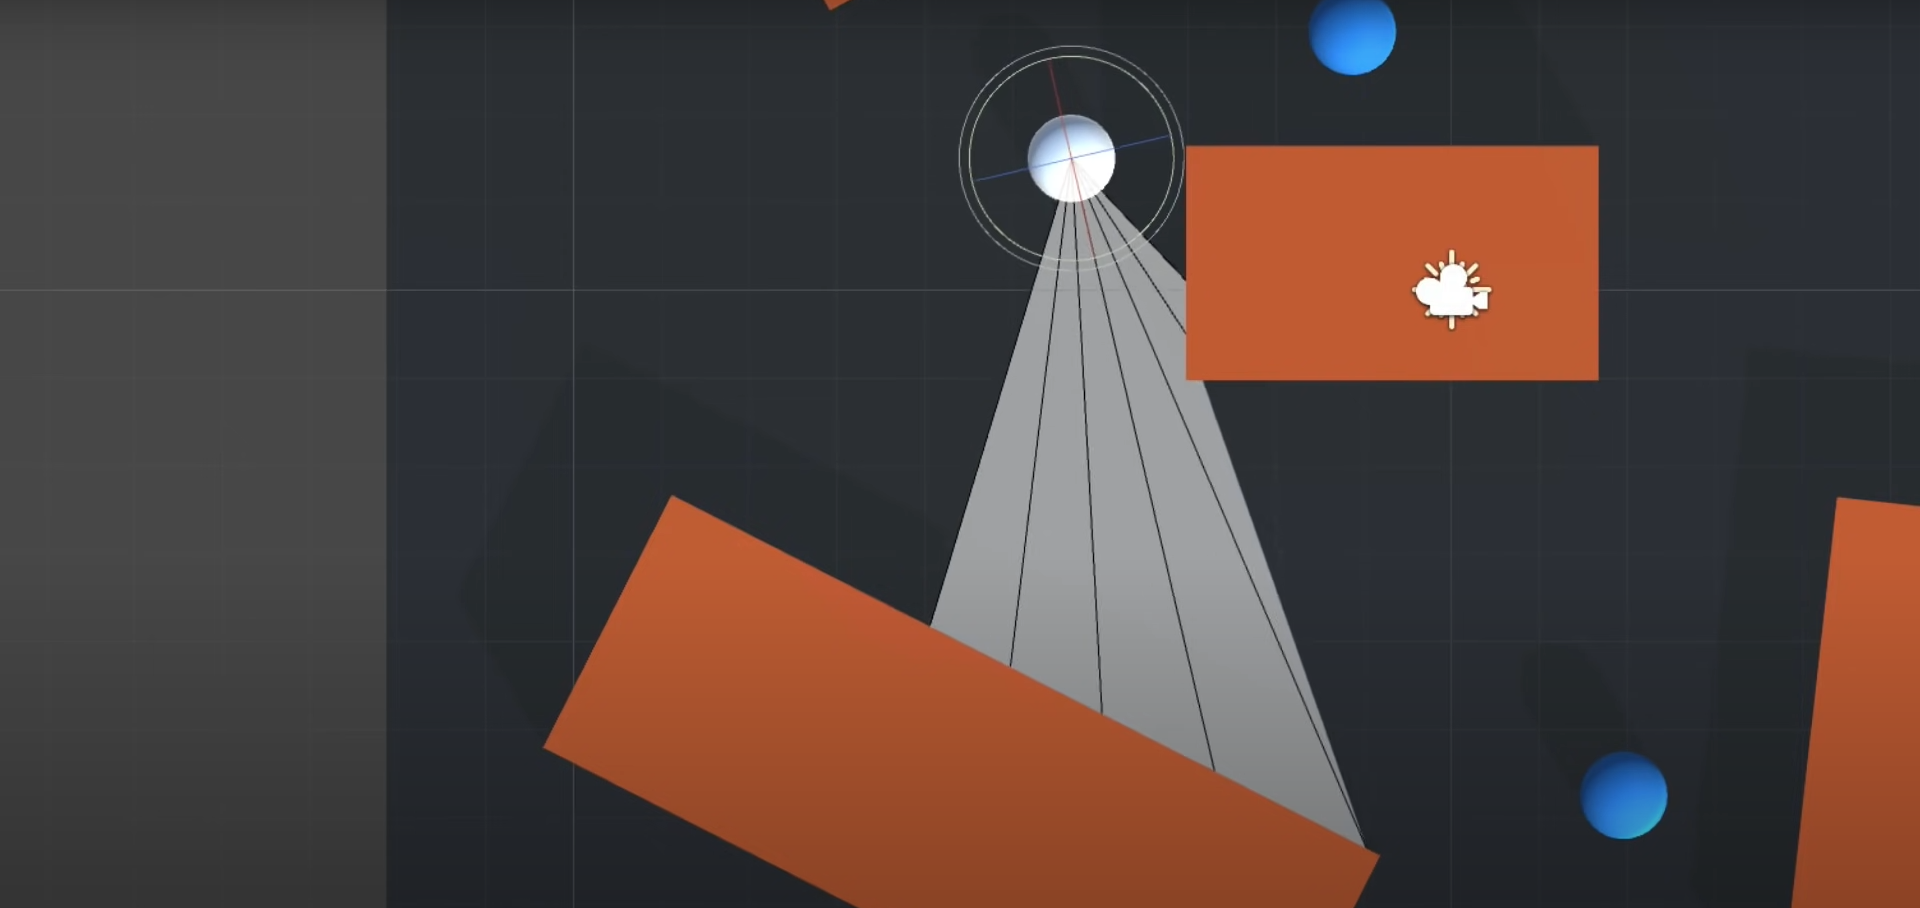
\includegraphics[width=1\columnwidth]{FOV(9).png} % Example image
	\caption{The binary search is not triggered and thus a falsely shaped triagle is formed in the mesh.}
\end{figure}

To solve the problem, the condition which triggers the solution of the edge problem was changed so that the solution is triggered either when a ray hits and the next one misses ending on the view radius, or two consecutive rays hit and the hit points are a distance apart greater than the EdgeDstThreshold (parameter set by the user). The result yields a smooth mesh, as that shown in Figure 9.

\begin{figure} % [h] forces the figure to be output where it is defined in the code (it suppresses floating)
	\centering
	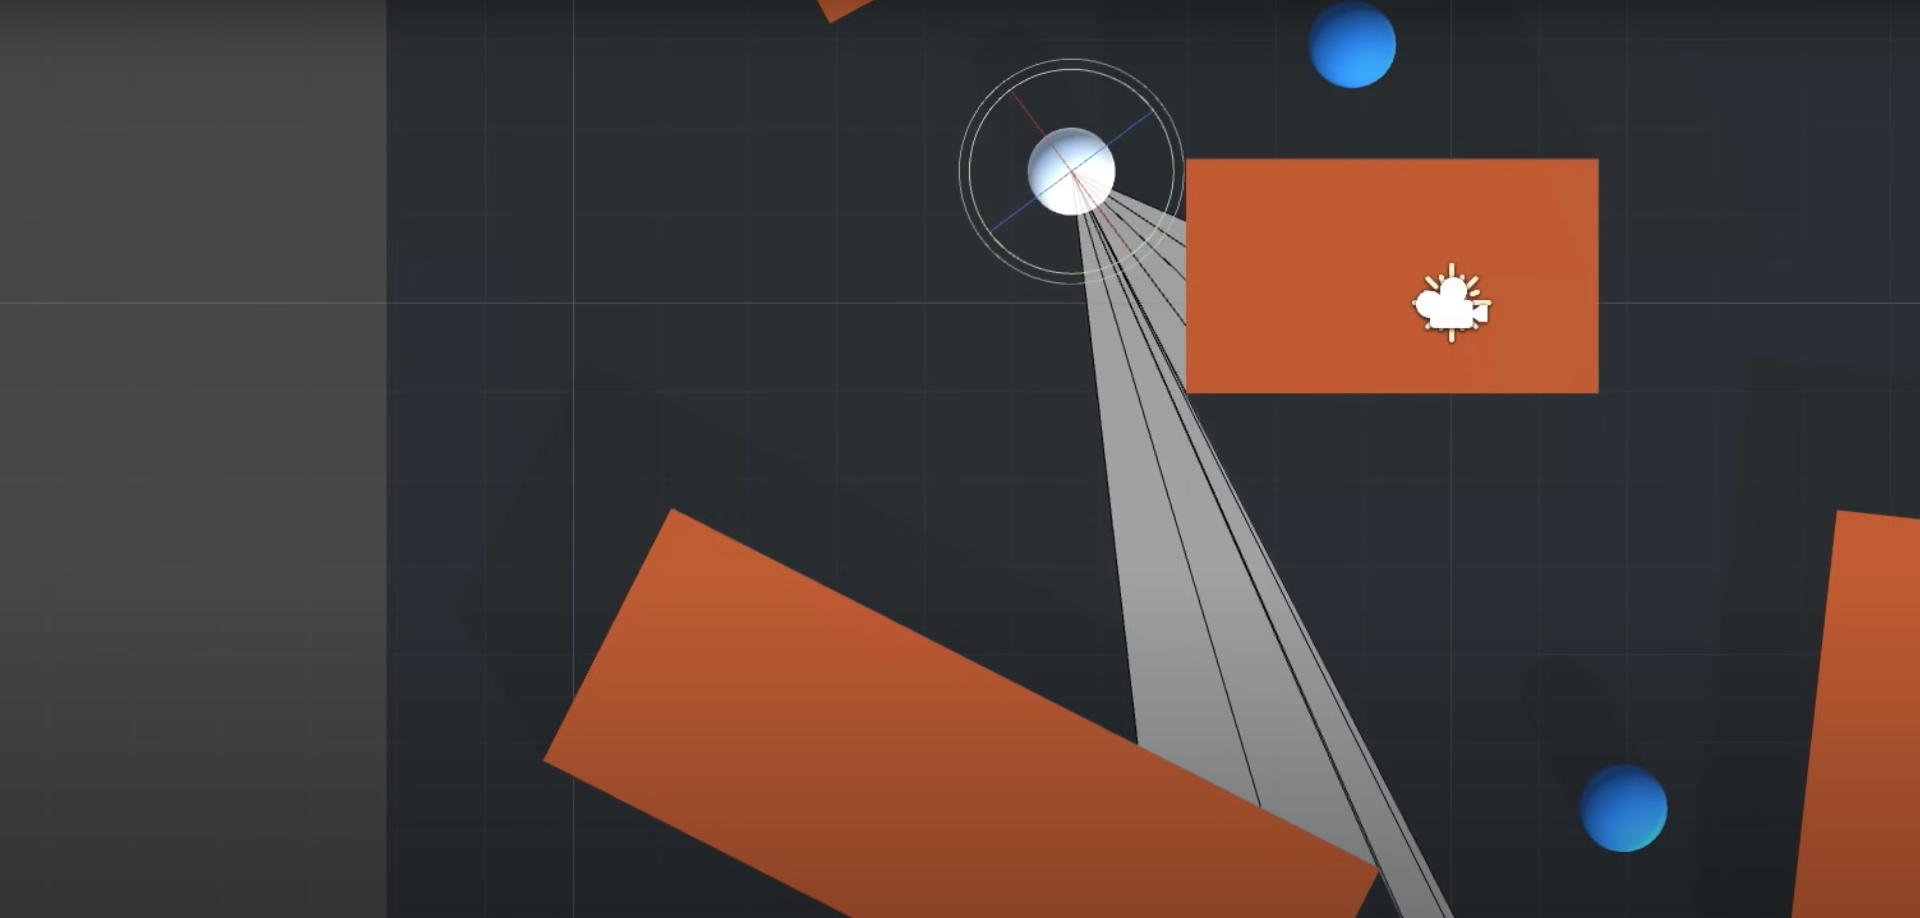
\includegraphics[width=1\columnwidth]{FOV(10).png} % Example image
	\caption{Smooth mesh after applying the edge problem solution.}
\end{figure}

The pseudo-code for the edge problem solution is shown in Algorithm 1.

\begin{algorithm}
\caption{EdgeProblemSolution}
\begin{algorithmic} 
\REQUIRE (previous ray hits $ \AND $  next ray does not hit) $ \OR $ (previous ray hits $ \AND $ next ray hits $ \AND $ next ray endpoint distance > EdgeDstThreshold)
\ENSURE There exists a ray that passes close enough to the obstacle edge.
\STATE $min \leftarrow angleOfRayThatHit$
\STATE $max \leftarrow angleOfRayThatMissed$
\STATE $i \leftarrow 1$
\WHILE{$i \leq EdgeResolveIterations$}
\STATE $ angle \leftarrow (min + \frac{max-min}{2}) $
\STATE $ Cast\; newRay\; with\; angle,\; min < angle < max$
\STATE $angleOfNewRay \leftarrow newRay.angle$
\IF{$newRay$ hits}
\STATE $min \leftarrow angleOfNewRay$
\ELSE
\STATE $max \leftarrow angleOfNewRay$
\ENDIF
\ENDWHILE
\STATE $ Add\: newRay.endpoint\; to\; the\; mesh $
\end{algorithmic}
\end{algorithm}

\subsection{Forming a 3D Mesh}

To form a 3D Mesh, multiple 2D Meshes, rotated around the appropriate axis were utilized. Namely, rotating horizontal meshes around the sensor's x-axis by a specific angle (horizontal offset) simulates a lidar's scanning slices created by the laser's horizontal motion (Figure 10a). Thus, a 3D mesh is created. To make the 3D mesh denser, the HorizontalOffsetResolution parameter can be increased. Similarily, rotating vertical meshes around the sensor's y-axis by a specific angle (vertical offset)  simulates a lidar's scanning slices created by the laser's vertical motion (Figure 10b).  To make the 3D mesh denser, the VerticalOffsetResolution parameter can be increased (Figure 10c).

\begin{figure}
\centering
\begin{subfigure}[b]{1\textwidth}
   \centering
   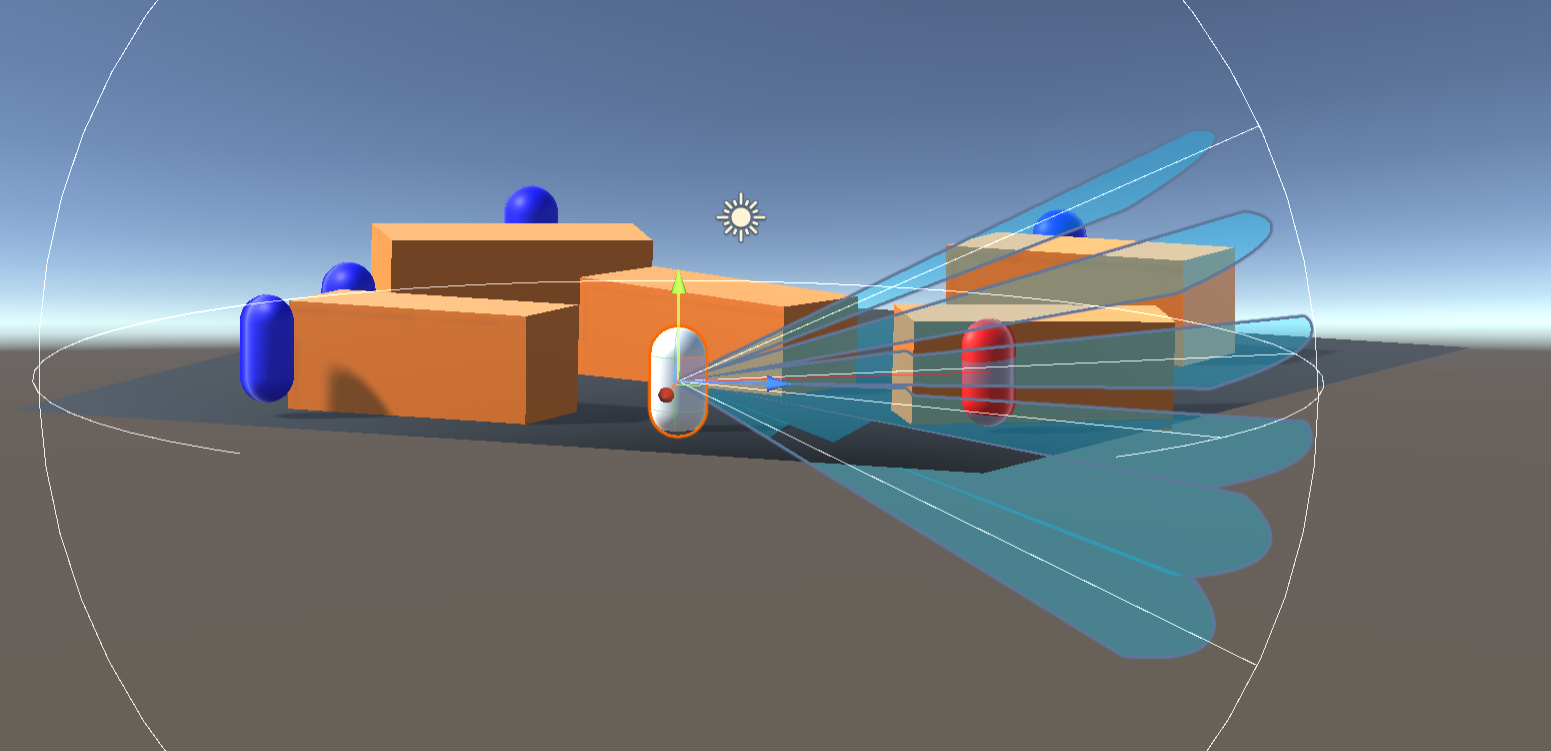
\includegraphics[width=0.8\linewidth]{FOV(11).png}
   \caption{Rotating horizontal meshes (side view).}
\end{subfigure}
\begin{subfigure}[b]{1\textwidth}
   \centering
   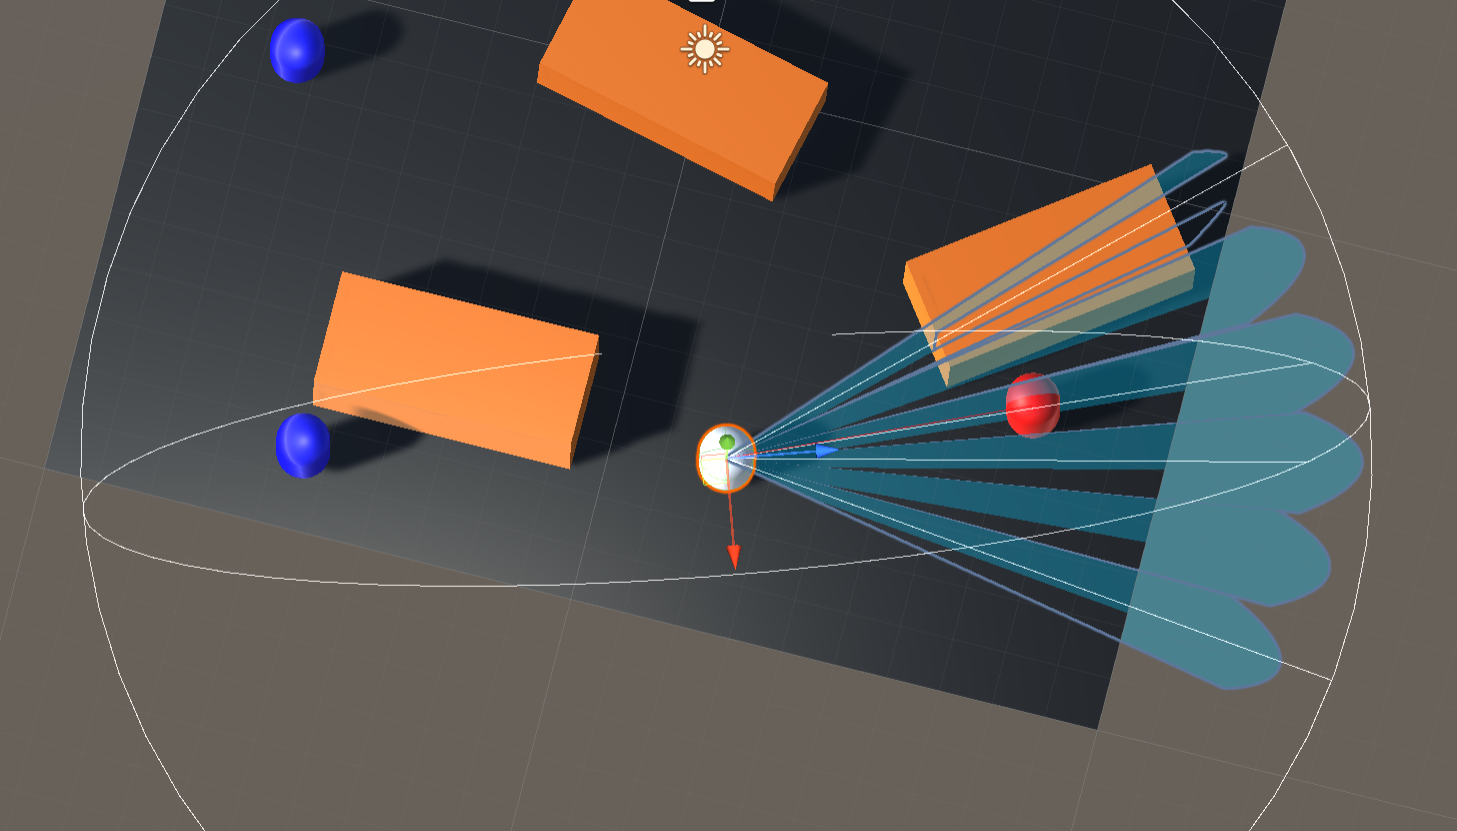
\includegraphics[width=0.8\linewidth]{FOV(12).png}
   \caption{Rotating vertical meshes (top view).}
\end{subfigure}
\begin{subfigure}[c]{1\textwidth}
   \centering
   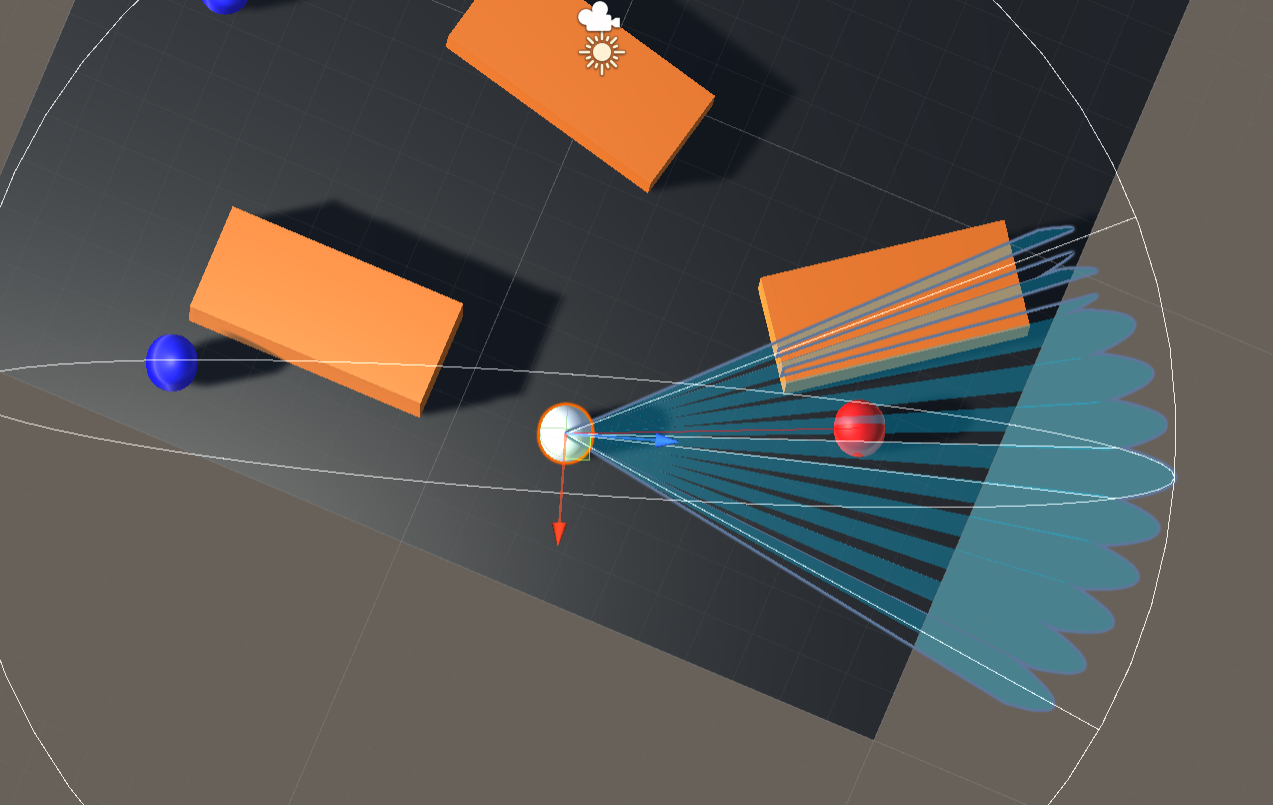
\includegraphics[width=0.8\linewidth]{FOV(13).png}
   \caption{Doubling the VerticalOffsetResolution.}
\end{subfigure}
\caption[]{Creating a 3D Mesh by rotating multiple 2D meshes.}
\end{figure}

The rotation of each mesh is achieved by rotating the rays that are casted to create it. The rays need to be rotated relative to the sensor's transform. For each ray there is a vector3 variable that determines its direction. It is easier to use rotation matrices to rotate each vector around the desired sensor axis \cite{noauthor_rotation_2022}. The matrix of a proper rotation R by angle $\theta$ around the axis $u = (u_x, u_y, u_z)$, a unit vector with $ u_x^2 + u_y^2 + u_z^2 = 1 $ is given by:
\\

$
\begin{bmatrix}
cos \theta + u_x^2(1 - \cos \theta) & u_xu_y(1 - \cos \theta)  - u_z\sin \theta & u_xu_z(1 - \cos \theta) + u_y\sin \theta
\\
u_yu_x(1 - \cos \theta) + u_z\sin \theta & \cos \theta + u_y^2(1 - \cos \theta) & u_yu_z(1 - \cos \theta) - u_x\sin \theta
\\
u_zu_x(1 - \cos \theta) - u_y\sin \theta & u_zu_y(1 - \cos \theta) + u_x\sin \theta & \cos \theta + u_z^2(1 - \cos \theta) 
\end{bmatrix}
$
\\

To form a denser and uniform 3D mesh, the rotation of both vertical and horizontal 2D meshes is necessary. Rotating horizontal meshes around the sensor's x-axis by a specific angle (horizontal offset) and vertical meshes around the sensor's y-axis by a specific angle (vertical offset) simulates a lidar's scanning slices created by the laser's horizontal and vertical motion. The resulting field of view closely resembles the geometry of a depth camera field of view (Figure 11a).

To make a uniform 3D mesh denser, the VerticalOffsetResolution parameter, the HorizontalOffsetResolution parameter or both parameters can be increased (Figure 11b).

This type of field of view visualization is the most accurate of those discussed so far and can be used to assist with decisions regarding a robot's perception system. 

\begin{figure}
\centering
\begin{subfigure}[b]{1\textwidth}
   \centering
   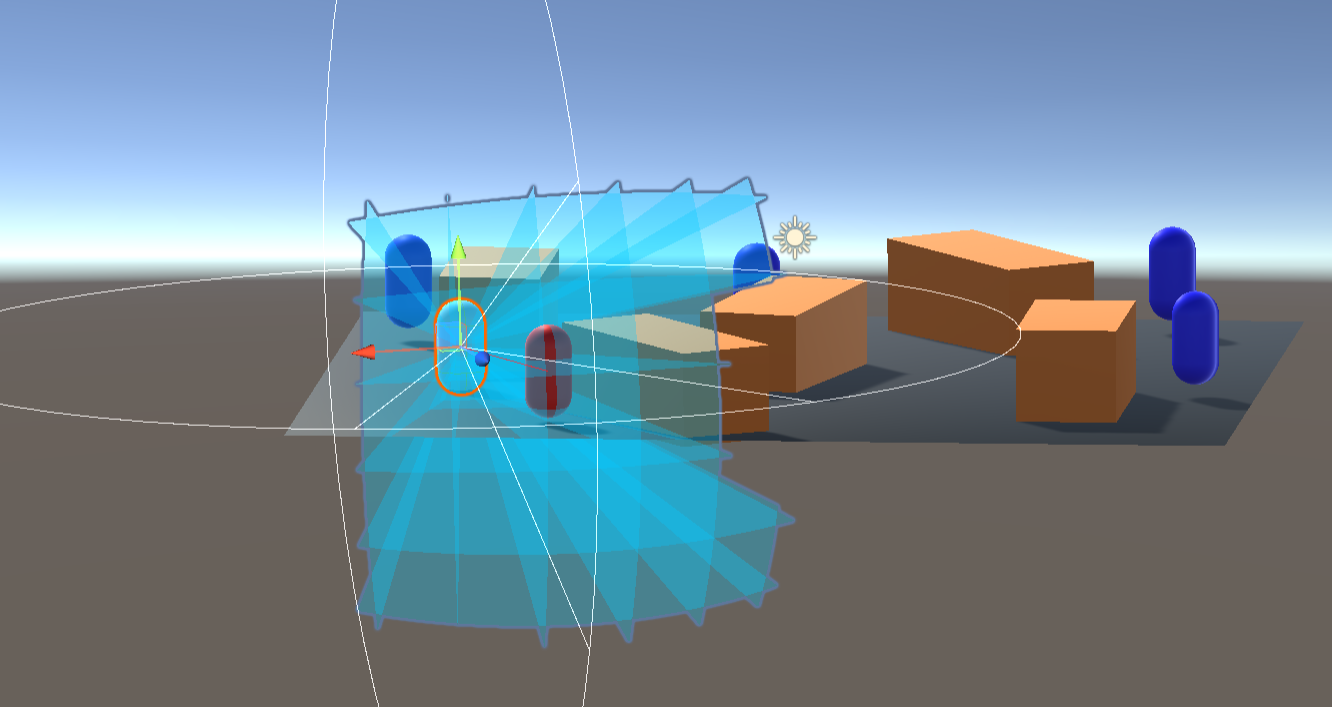
\includegraphics[width=0.8\linewidth]{FOV(14).png}
   \caption{Dense enough uniform 3D mesh (front view).}
\end{subfigure}
\begin{subfigure}[b]{1\textwidth}
   \centering
   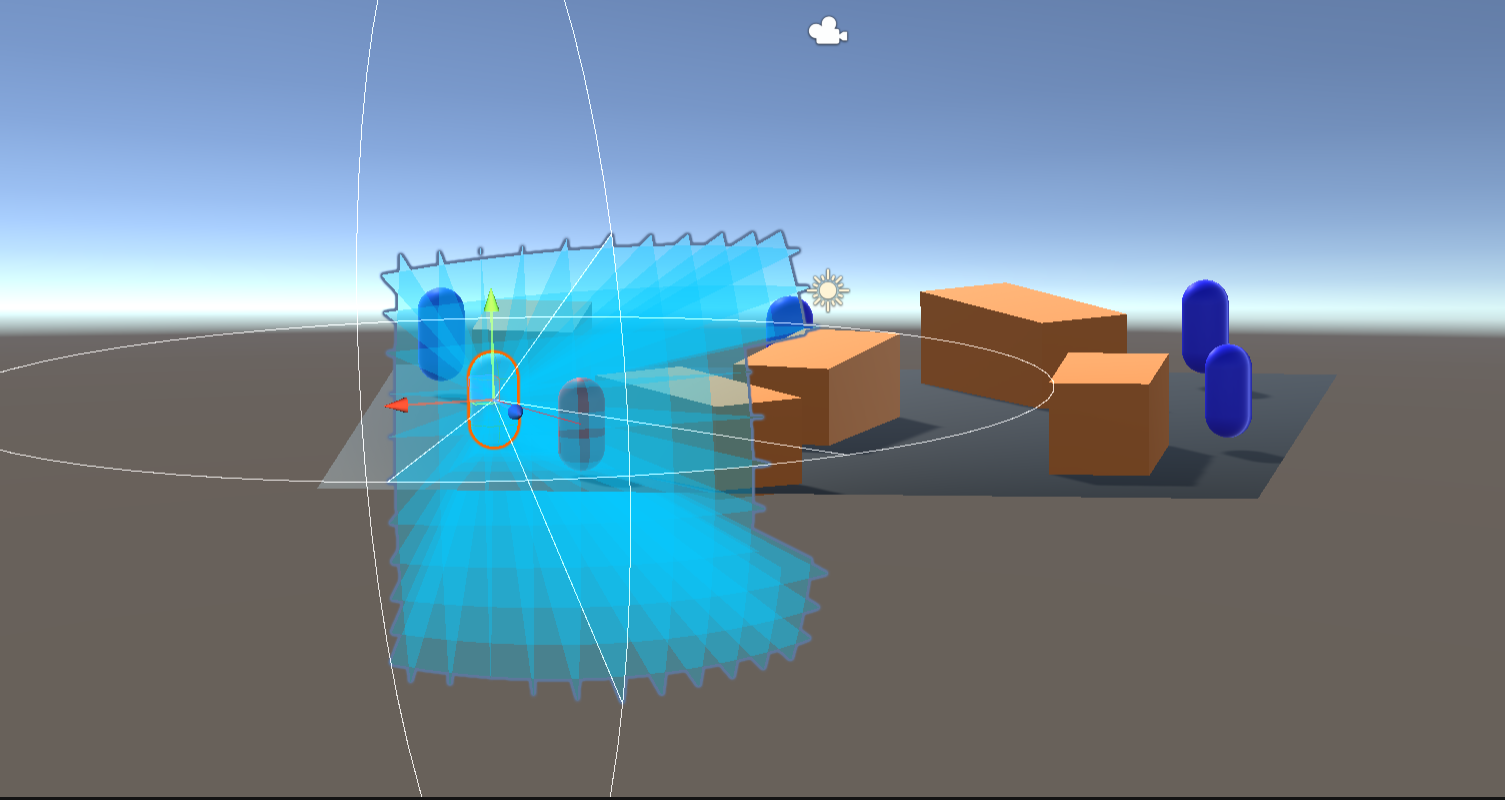
\includegraphics[width=0.8\linewidth]{FOV(15).png}
   \caption{Denser uniform 3D mesh (front view).}
\end{subfigure}
\caption[]{3D meshes formed by rotating horizontal and vertical meshes.}
\end{figure}



\subsection{Detecting Visible Targets}

The blue capsules in the scene represent targets. Targets that are in the overall field of view of the robot's perception system are marked with red color instead of blue. The information that a target is inside the overall field of view can be acquired in two ways:
The first one is utilizing the rays that are casted to form the 2D meshes. A check can be run for each ray to determine if the ray hits a target or not. If a target is hit, it can then be marked as visible and it can be added to a list containing all the visible targets. In an editor script, the red color can be assigned to every target in the list with the visible targets. 
This method simulates a lidar's visibilty constraints. It can test a lidar's vertical and horizontal resolution. Namely, if a target's dimensions are smaller than the dimension of a single cell in the 3D mesh grid formed by the rays, then the target could remain undetected even if its position is in the sensor's effective field of view, as seen in Figure 12. This test case simulates a lidar that is unable to map a small object or detail despite the latter being inside the lidar's declared field of view.

\begin{figure} % [h] forces the figure to be output where it is defined in the code (it suppresses floating)
	\centering
	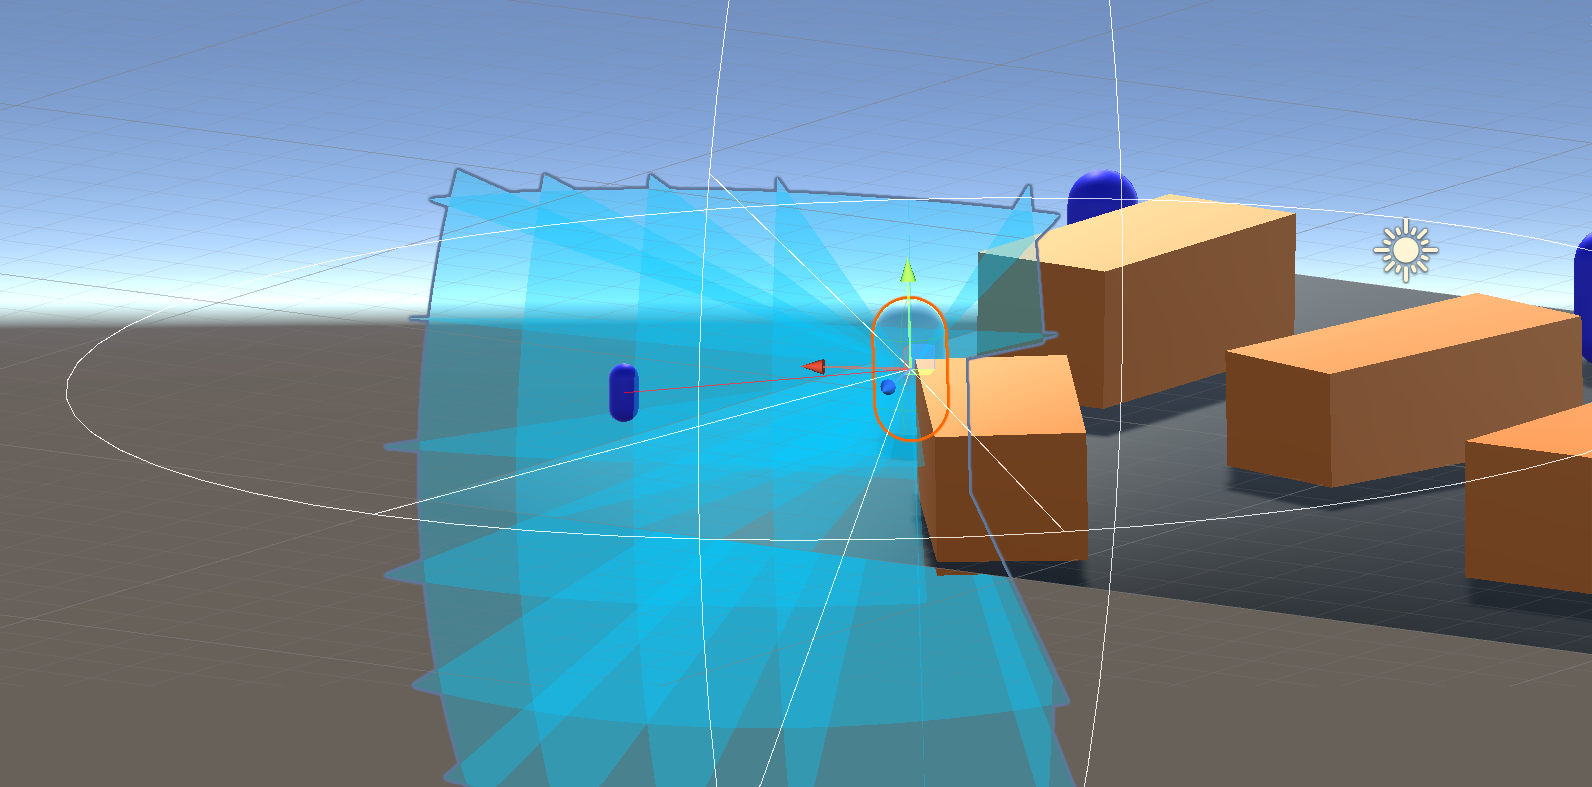
\includegraphics[width=1\columnwidth]{FOV(16).png} % Example image
	\caption{Capsule target is positioned in the effective field of view but is too small to be detected by the sensor. Thus it is not colored in red.}
\end{figure}

The second way to acquire the information that a target is inside the overall field of view, is to simply use math to check if the center of the target lies within the field of view locus. For that to be true, three conditions have to be met. 
\begin{itemize}
    \item The distance between the sensor's center and the target's center must be smaller than the view radius.
    \item The angle formed by the sensor's z transform vector (front vector) and the projection of the target's relative position vector to the sensor's $\overrightarrow{\text{y}}$ plane ($a$), must be smaller than the horizontalViewAngle ($hova$). This is visualized in Figure 13a.
    \item The angle formed by the sensor's z transform vector (front vector) and the projection of the target's relative position vector to the sensor's $\overrightarrow{\text{x}}$ plane ($b$), must be smaller than the verticalViewAngle ($veva$). This is visualized in Figure 13b.
\end{itemize}

\begin{figure}
\centering
\begin{subfigure}[b]{1\textwidth}
   \centering
   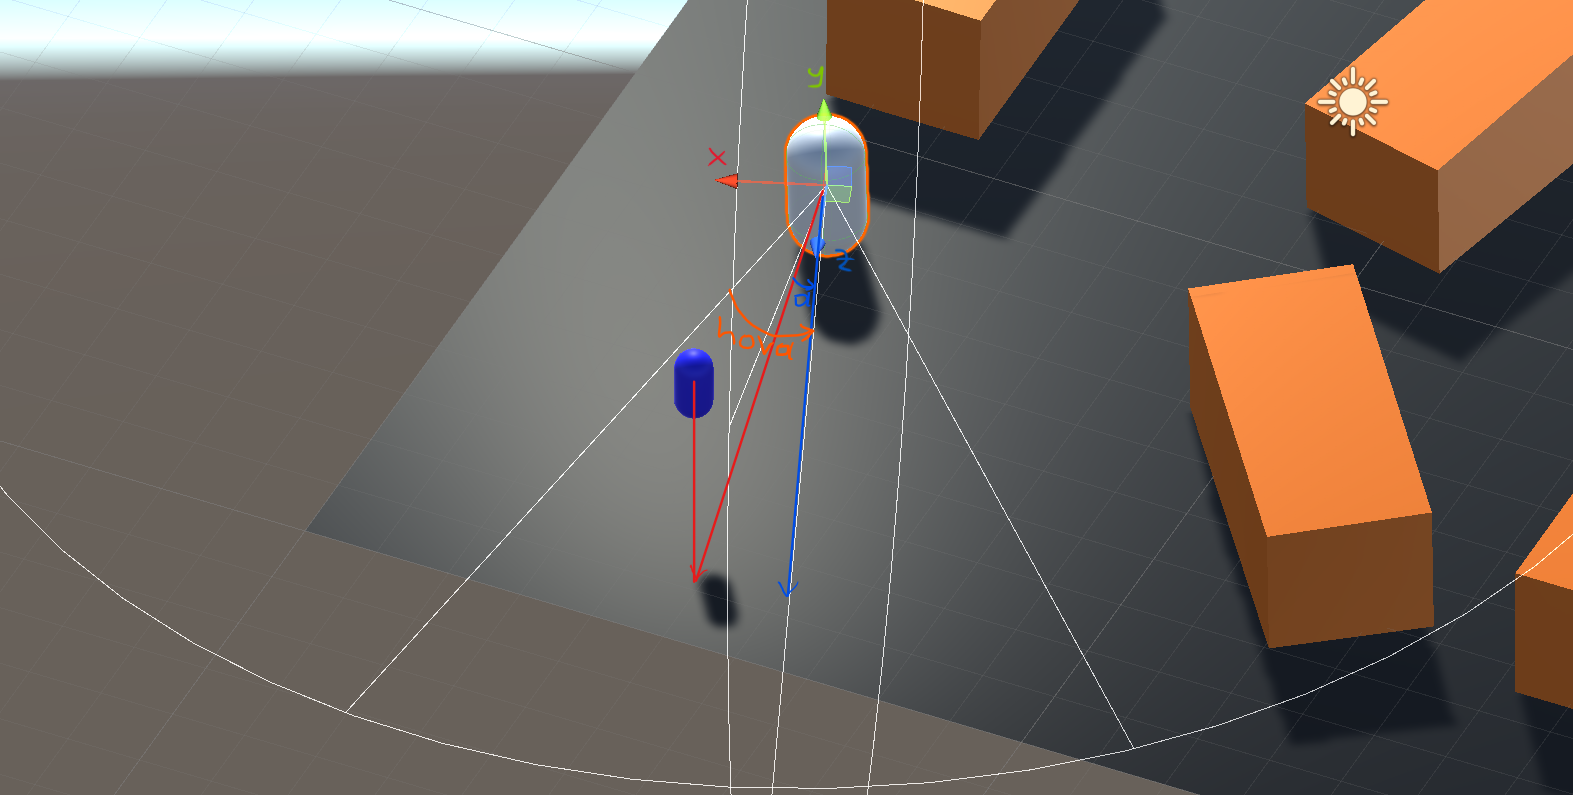
\includegraphics[width=0.8\linewidth]{FOV(17).png}
   \caption{Projection of the target's relative position vector to the sensor's $\overrightarrow{\text{y}}$ plane}
\end{subfigure}
\begin{subfigure}[b]{1\textwidth}
   \centering
   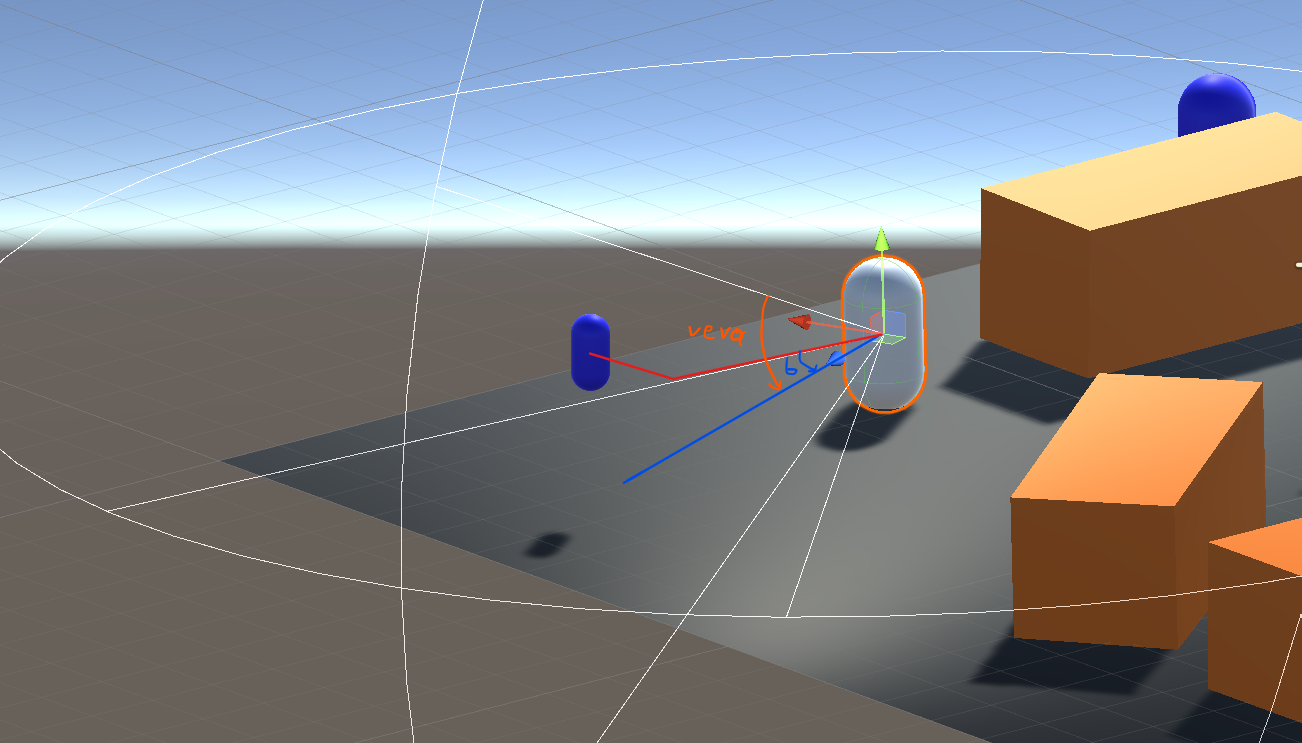
\includegraphics[width=0.8\linewidth]{FOV(18).png}
   \caption{Projection of the target's relative position vector to the sensor's $\overrightarrow{\text{x}}$ plane}
\end{subfigure}
\caption[]{Using the field of view locus method to check that a target is visible.}
\end{figure}

This method simulates a camera's visibility effectiveness, if it is assumed that the camera has no blind spots. 

\clearpage


\section{The laelaps perception system}

\subsection{Perception system requirements}

To determine the ideal position and rotation of the sensors on the laelaps robot, a list of specific requirements was considered. These requirements resulted from the intended use of the robot, namely  in outdoor agricultural environments and more specifically in vineyards for grape and vine inspection. Naturally, each of these requirements cannot always be fulfilled and therefore, trade-offs play an essential role when designing 3D perception systems. In summary, the 3D perception system requirements for the laelaps robot are shown in Table 1. 

\begin{table}[htbp]
\centering
\begin{tabular}{ | m{1cm} | m{10cm}| } 
  \hline
  \textbf{index} & \textbf{Requirement} \\ 
  \hline
  1 & The 3D perception system should have the best possible observation area and the least possible blind spots. \\ 
  \hline
  2 & The 3D perception system should be energy efficient. \\ 
  \hline
  3 & The view radius of the robot should be large enough for the robot to detect obstacles early enough to avoid them. \\ 
  \hline
  4 & The vision of the robot should not be heavily impaired under adverse weather or lighting conditions. \\ 
  \hline
  5 & The 3D perception system should be capable of distinguishing visual features and areas of interest in ranges of at least up to two meters.  \\ 
  \hline
  6 & The 3D perception system should be capable of mapping ground terrain well enough to distinguish incline and ground uneveness or irregularities which should be avoided. \\ 
  \hline
  7 & The 3D perception system should be capable of mapping whole vines and similar plants which can reach more than a meter in height. \\ 
  \hline
\end{tabular}
\caption{Summary of 3D perception system requirements.}
\end{table}


\subsection{Discussing possible sensor configurations}

With these requirements in mind, seven different sensor configurations for the laelaps 3D perception system were tested using the Field of view visualization tool in unity.

\begin{enumerate}
\item Laelaps with 2x Zed2 Cameras \cite{noauthor_zed_nodate} and a Velarray M1600 Lidar \cite{noauthor_velarray_nodate}.

This option offers a large observation area covering the whole front and sides of the robot, with small and not substantial blind spots (Figure 14). However, there is no view from the back of the robot, which could be useful in case the performs maneuvers which require it to move backwards. An extra Zed2 stereo camera could be added at the back of the robot providing the setup with a near 360$^{\circ}$ field of view.
In terms of energy efficiency, this setup is lightweight and efficient. The ZED2 cameras consume a mere 380 mW each while the Velarray M1600 Lidar, being a solid state lidar with no moving parts, needs 11 W at most to be fully operational. Combining lidars and depth cameras allows for versatility even in adverse weather or lighting conditions. Lidars do not require external light sources to operate and their functionality is not affected by changes in lighting conditions. Cameras on the other hand are generally not as susceptible to rain, fog or dust as lidars. They can also map reflective surfaces with more accuracy than lidars. However, given that the field of view of the cameras does not overlap with the field of view of the lidar, if a sensor underperforms then the whole system is affected. 

\begin{figure}
\centering
\begin{subfigure}[htbp]{1\textwidth}
   \centering
   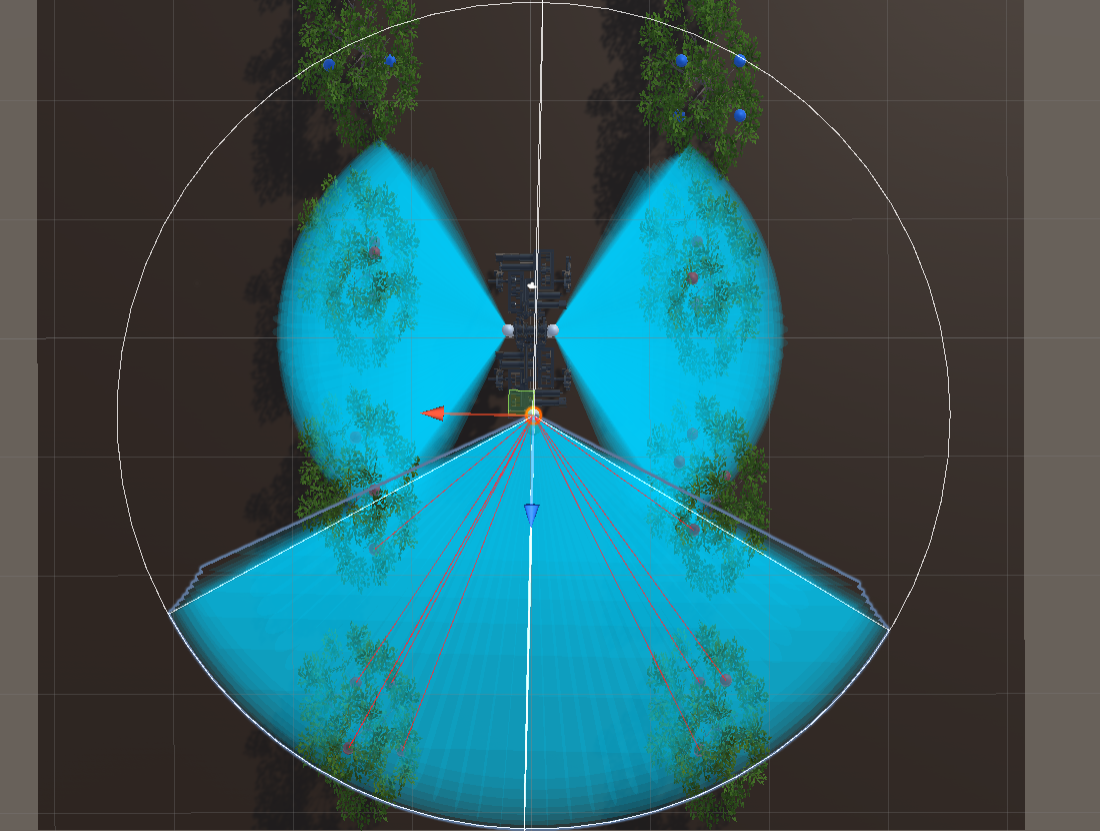
\includegraphics[width=0.8\linewidth]{FOV(19).png}
   \caption{Top view of Lealaps with 2x Zed2 Cameras and a Velarray M1600 Lidar.}
\end{subfigure}
\begin{subfigure}[htbp]{1\textwidth}
   \centering
   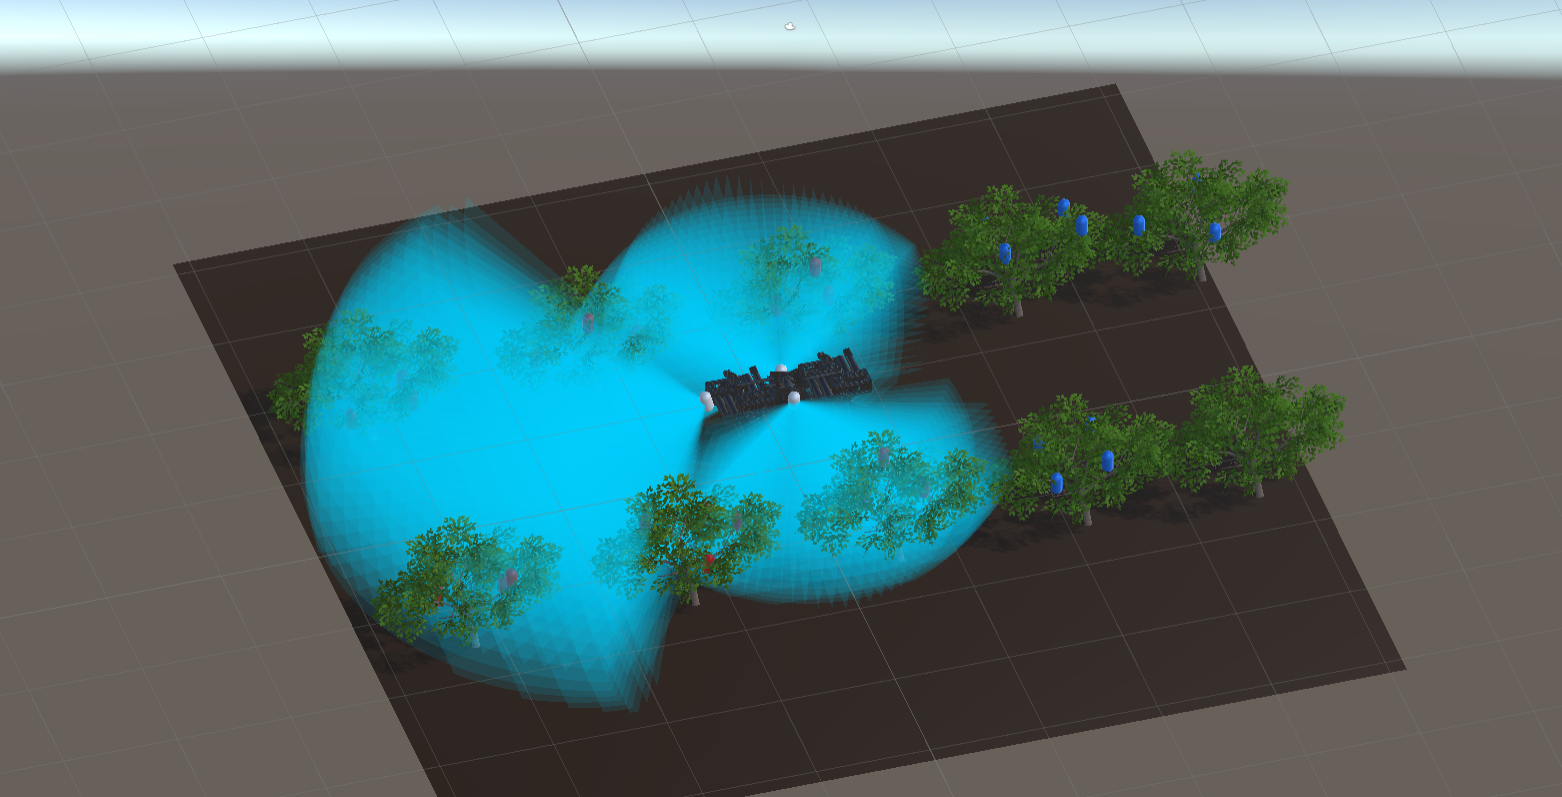
\includegraphics[width=0.8\linewidth]{FOV(20).png}
   \caption{Side view of Lealaps with 2x Zed2 Cameras and a Velarray M1600 Lidar.}
\end{subfigure}
\caption[]{Using the FOV\_Visualizing tool in unity to check for blind spots and overall visibility constraints.}
\end{figure}


\item Laelaps with 4x Intel Realsense D435 depth Cameras \cite{noauthor_depth_nodate}. 

This option also offers a large observation area covering the whole front, sides and back of the robot, with small although not negligible blind spots (Figure 15). In addition, the D435 depth cameras offer a large vertical field of view angle (58$^{\circ}$), which allows the robot to easily obtain depth images of tall plants, even when standing close to them. 
In terms of energy efficiency, this setup is lightweight and very efficient. The maximum power draw of the Vision Processor D4 Board, which handles power for both the Vision Processor D4 and the Depth Module of the D435 camera, is rated at 700 mA. With a nominal supply voltage of 5V, each camera consumes a mere 3.5W for a total of 14W for the whole setup. 
Nevertheless, this setup utilizes only depth cameras. The absence of a lidar means that the field of view radius or the effective range of the perception sensors is smaller, while the pointcloud quality at the front side of the robot would be inferior as lidars do produce higher quality and relatively artifact-free depth-clouds.

\begin{figure}
\centering
\begin{subfigure}[htbp]{1\textwidth}
   \centering
   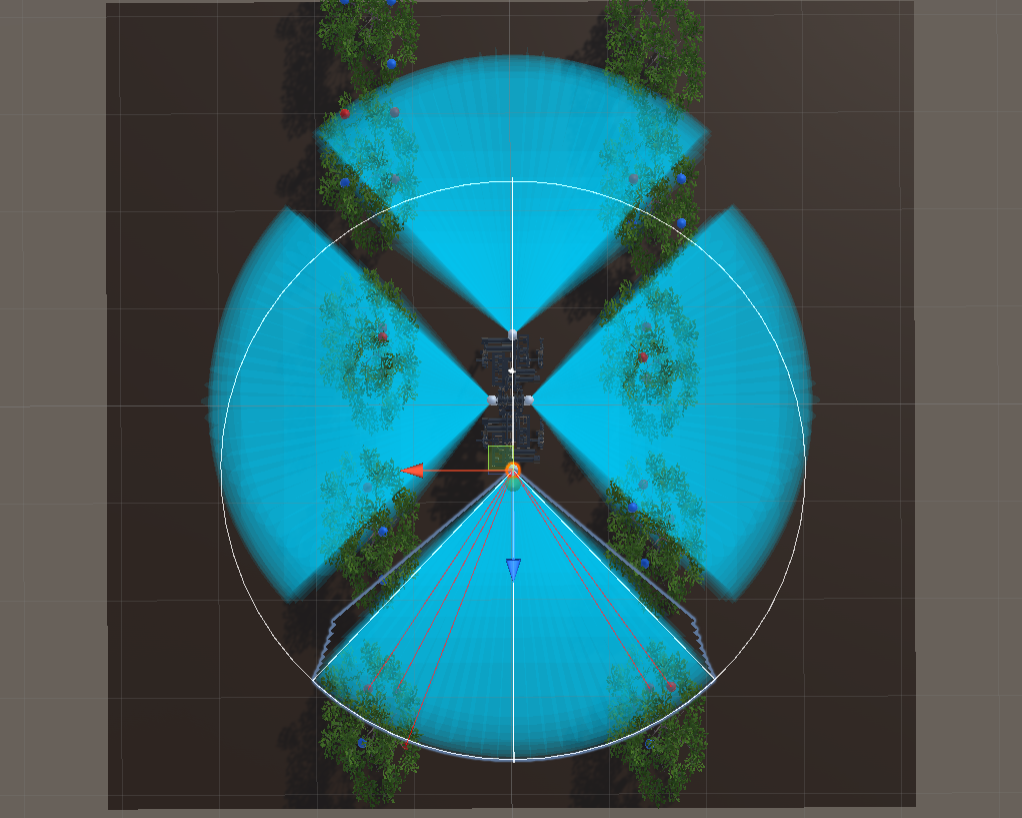
\includegraphics[width=0.8\linewidth]{FOV(21).png}
   \caption{Top view of Lealaps with 4x Intel Realsense D435 depth Cameras.}
\end{subfigure}
\begin{subfigure}[htbp]{1\textwidth}
   \centering
   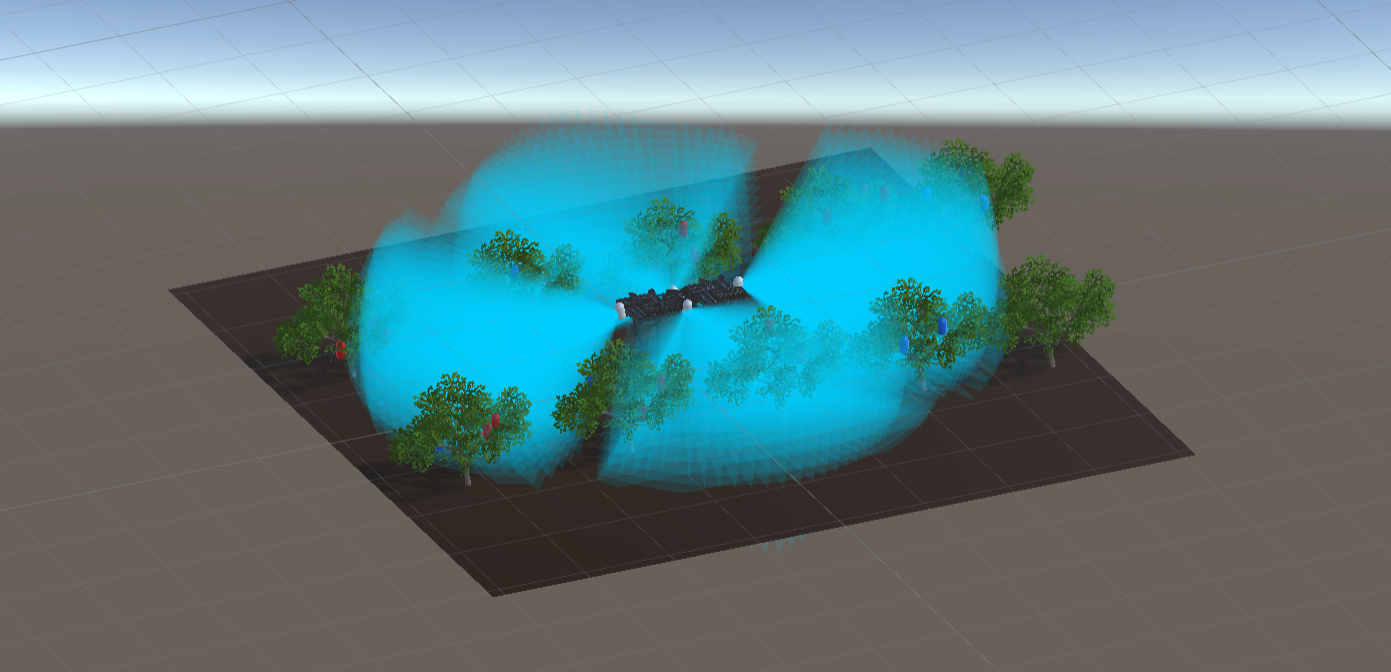
\includegraphics[width=0.8\linewidth]{FOV(22).png}
   \caption{Side view of Lealaps with 4x Intel Realsense D435 depth Cameras.}
\end{subfigure}
\caption[]{Using the FOV\_Visualizing tool in unity to check for blind spots and overall visibility constraints and capabilities.}
\end{figure}

\item Laelaps with 5x Intel Realsense D435 depth Cameras. 

An interesting approach to keeping the simplicity and energy efficiency of the second setup, while raising the depth-cloud quality at the same time is adding a fifth Intel Realsense D435 sensor. Since most obstacles and points/areas of interest will appear in front of the robot, the extra camera should be placed on the front side of the robot, alongside the preexisting front depth camera. In this particular approach, the two front cameras are rotated around the y-axis, which in unity is the vertical axis,at 20$^{\circ}$ inward so that their field of views overlap (Figure 16). This creates information redundancy but yields a higher quality depth-cloud overall, since a single underperforming front sensor (for example due to dust or strong direct light on the lenses) will not affect the generated front depth map. 
This setup, nevertheless, does not increase the effective range of the robot's perception. It does, however, reduce the size of the blind spots on the front side of the overall field of view. Boston Dynamic's spot robot utilizes a similar perception system \cite{noauthor_about_nodate}.

\begin{figure}
\centering
\begin{subfigure}[htbp]{1\textwidth}
   \centering
   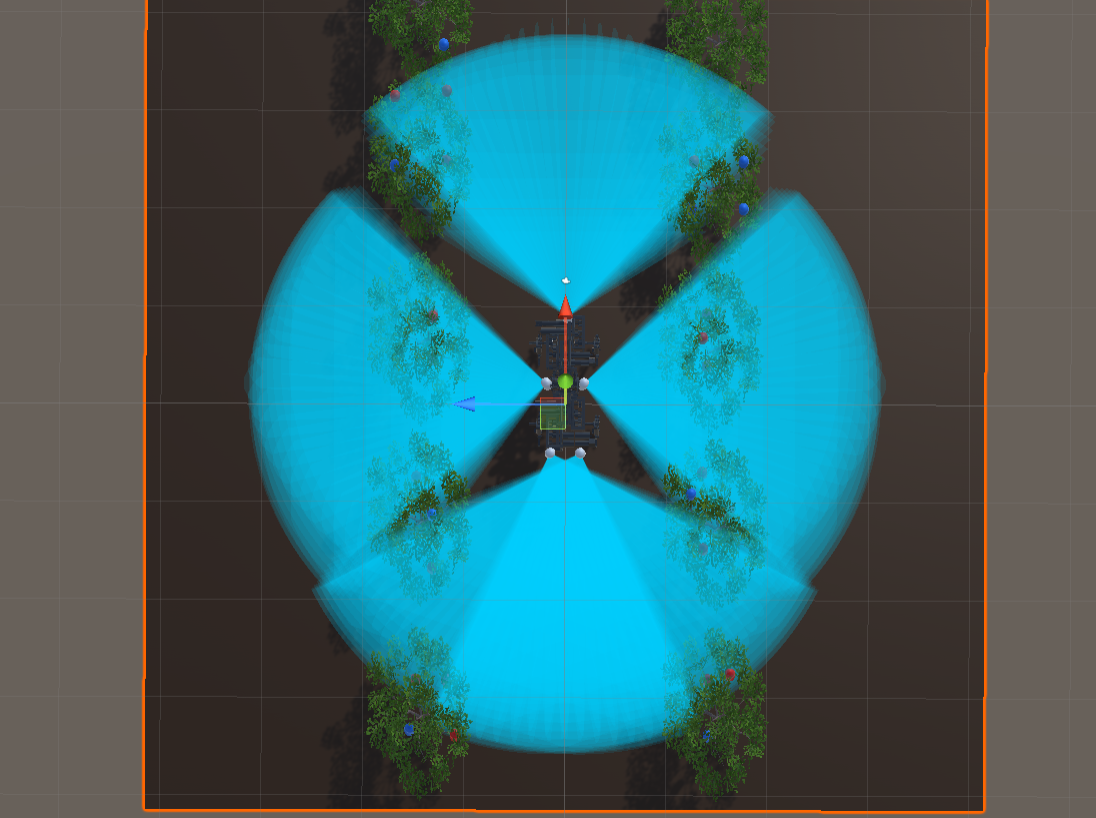
\includegraphics[width=0.8\linewidth]{FOV(23).png}
   \caption{Top view of Lealaps with 5x Intel Realsense D435 depth Cameras.}
\end{subfigure}
\begin{subfigure}[htbp]{1\textwidth}
   \centering
   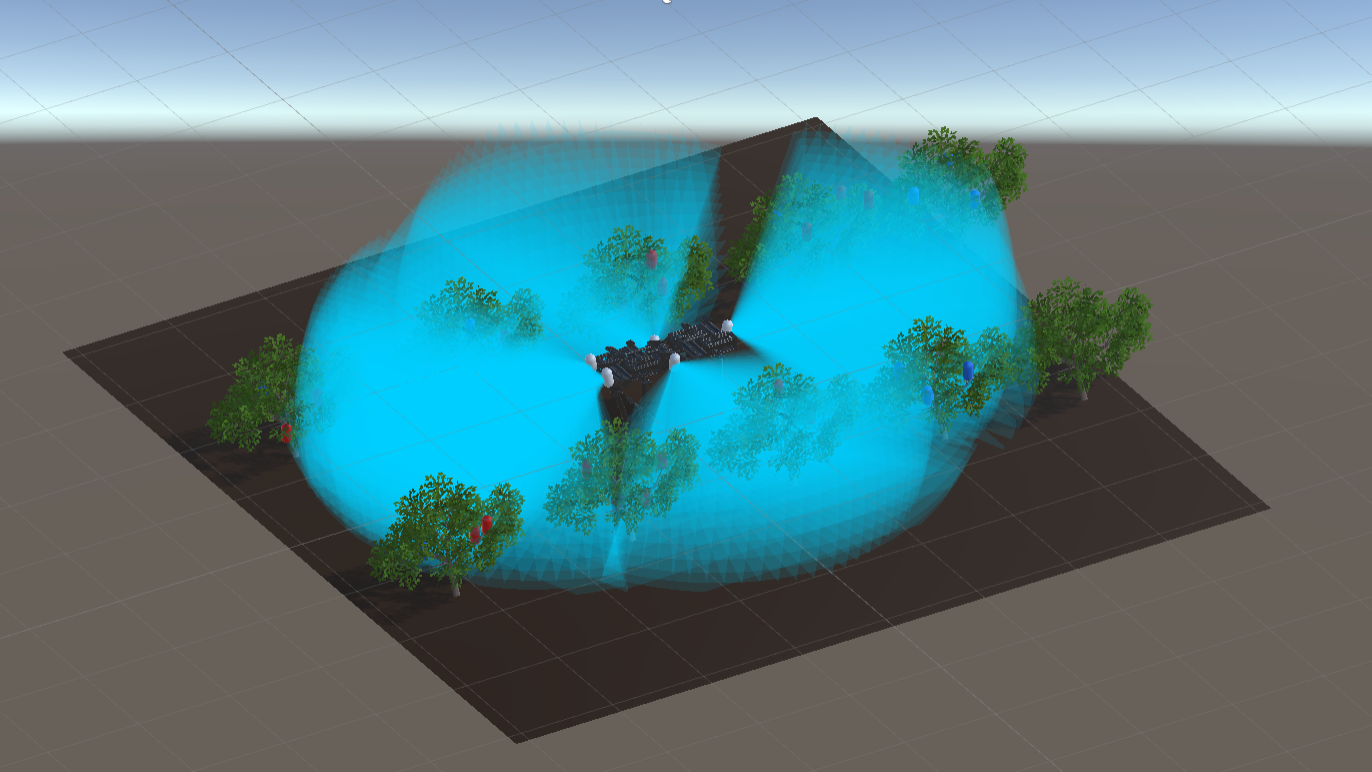
\includegraphics[width=0.8\linewidth]{FOV(24).png}
   \caption{Side view of Lealaps with 5x Intel Realsense D435 depth Cameras.}
\end{subfigure}
\caption[]{Using the FOV\_Visualizing tool in unity to check for blind spots and overall visibility constraints and capabilities.}
\end{figure}

\clearpage

\item  Laelaps with 4xD435 + Velodyne Ultra Puck Surround View Lidar \cite{noauthor_ultra_nodate}.

Informational redundancy can lead to a more robust perception system. This approach utilizes overlapping 3D fields of view to accomplish just that. On the centre top of the robot, a Velodyne Ultra Puck Surround View Lidar offers a 360$^{\circ}$ field of view with high resolution. To refine the resulting pointcloud, 4xD435 depth cameras, one in every side of the robot, provide additional depth images. There are no blind spots with this setup (Figure 17) and an underperforming sensor will not significantly affect the produced pointcloud.
A major drawback of this system is the weight and the limited energy efficiency. The lidar alone is around 1kg heavy. It consumes 10W of power at typical operating conditions. This makes this perception system the heaviest and most energy-consuming system discussed so far. In addition, it is not focused on one particular side of the robot. The fiels of view expand evenly away from the robot. This is usually not desired, as four legged robots are generally more agile when moving forwards and thus it is a preferable design choice for the perception system to be focused on the front side of the robot. Anybotics Anymal C robot utilizes a similar perception system \cite{noauthor_anymal_nodate}.

\begin{figure}
\centering
\begin{subfigure}[htbp]{1\textwidth}
   \centering
   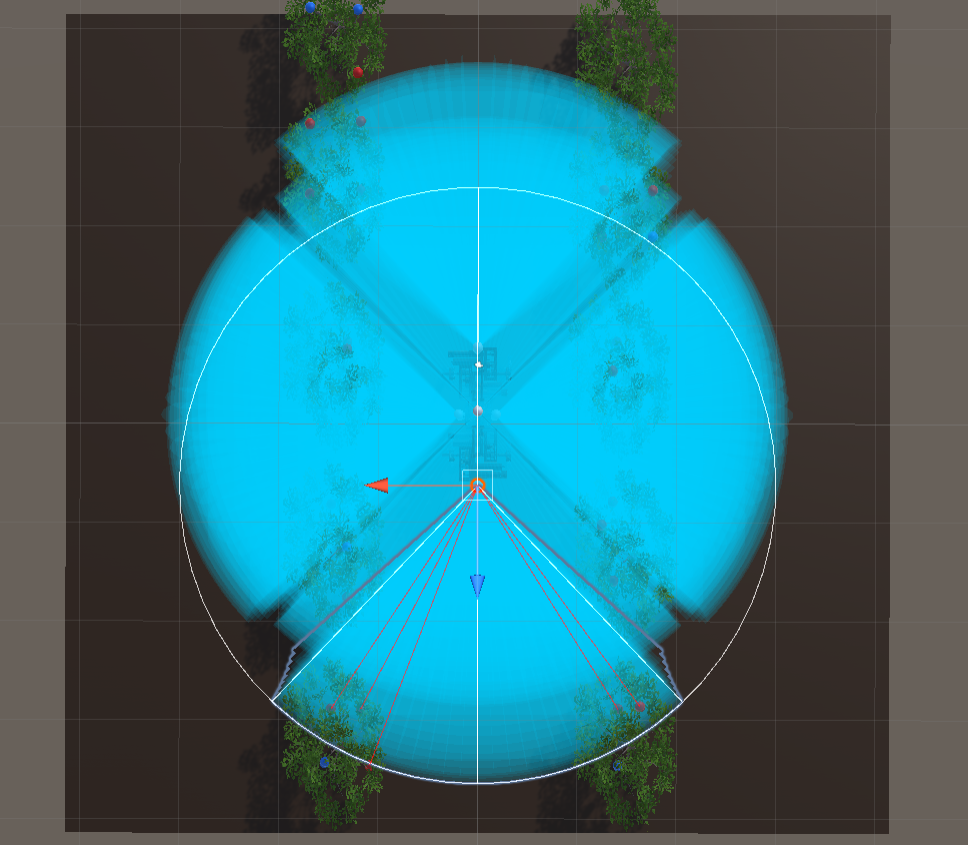
\includegraphics[width=0.8\linewidth]{FOV(25).png}
   \caption{Top view of Lealaps with 4x Intel Realsense D435 depth Cameras and a Velodyne Ultra Puck Surround View Lidar.}
\end{subfigure}
\begin{subfigure}[htbp]{1\textwidth}
   \centering
   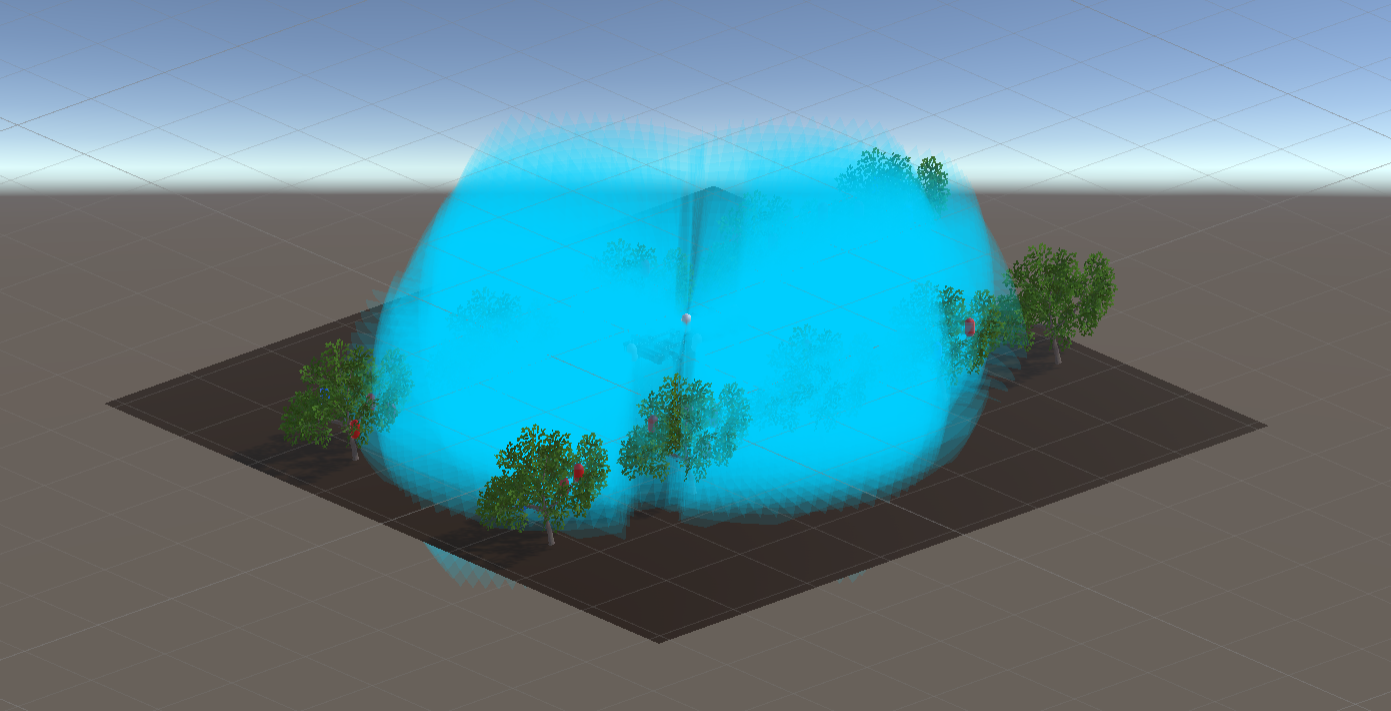
\includegraphics[width=0.8\linewidth]{FOV(26).png}
   \caption{Side view of Lealaps with 4x Intel Realsense D435 depth Cameras and a Velodyne Ultra Puck Surround View Lidar.}
\end{subfigure}
\caption[]{Using the FOV\_Visualizing tool in unity to check for blind spots and overall visibility constraints and capabilities.}
\end{figure}

\item  Laelaps with 4xD435 and an extra D435 at the front, rotated around the x-axis.

This configuration aims to improve the robot's perception in the front, while also improving the overall vertical field of view. Robots that will commonly encounter obstacles (e.g. branches) high above their body height or need to gather visual information from tall objects and structures will benefit from a design like this. Several -though not significant- blind spots appear when visualizing the overall field of view of this perception system (Figure 18). The small overlap between the two front camera's field of view will yield slightly better pointcloud quality in front of the robot. The system is very energy efficient and lightweight since it only utilizes lightweight depth cameras with low consumption (typically 3.5W).
Xiaomi's Cyberdog utilizes a similar setup, due to its need to have visual contact with human faces and gestures \cite{noauthor_xiaomi_nodate}.

\begin{figure}
\centering
\begin{subfigure}[htbp]{1\textwidth}
   \centering
   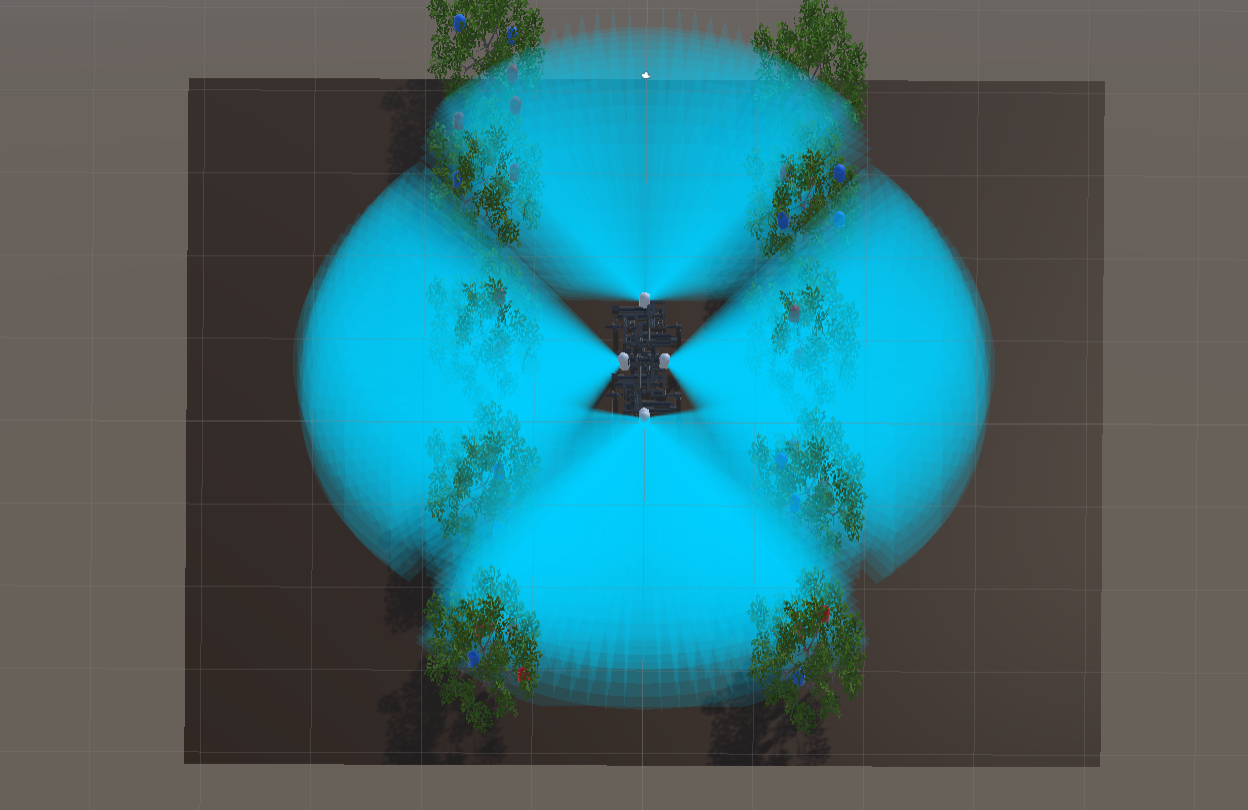
\includegraphics[width=0.8\linewidth]{FOV(27).png}
   \caption{Top view of Lealaps with 4x Intel Realsense D435 depth Cameras and an extra D435 at the front, rotated around the x-axis.}
\end{subfigure}
\begin{subfigure}[htbp]{1\textwidth}
   \centering
   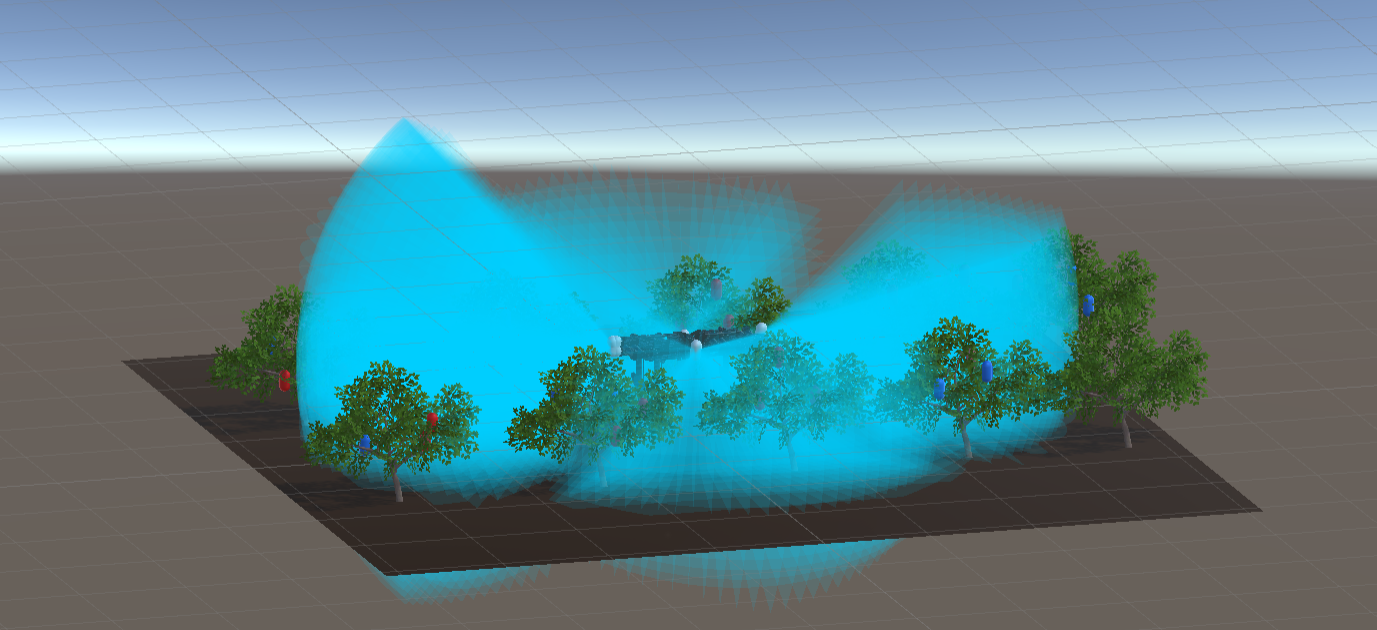
\includegraphics[width=0.8\linewidth]{FOV(28).png}
   \caption{Side view of Lealaps with 4x Intel Realsense D435 depth Cameras and an extra D435 at the front, rotated around the x-axis.}
\end{subfigure}
\caption[]{Using the FOV\_Visualizing tool in unity to check for blind spots and overall visibility constraints and capabilities.}
\end{figure}

\clearpage

\subsection{Deciding on a near optimal sensor configuration for Laelaps}

The Laelaps robot being optimally designed using a combination of criteria related to forward speed, would benefit from a perception system that is focused on the front of the robot. However, in agricultural environments, the robot will encounter difficult terrain, dead-ends and obstacles that cannot be easily avoided. In such conditions, the robot will be required to rotate, turn and even walk backwards. Therefore, the robot should be equipped with a setup that produces a near 360$^{\circ}$ field of view. Considering this, as well as the summary of 3D perception system requirements presented in Table 1, the Laelaps sensor configuration will consist of 4x ZED2 Stereo Depth cameras and one  Velarray M1600 Solid State Lidar. Combining a Lidar with depth cameras will provide versatility to the system and robustness even in adverse weather or lighting conditions. Placing the lidar on the front side of the robot and overlapping its field of view with that of the front depth camera will add to the existing robustness. Capitalising on the increased range of the lidar, the lidar is placed at a subtler downward angle than the front depth camera (Figure 19). Thus, the camera mainly maps the ground close and in front of the robot, while the lidar captures information about terrain and obstacles further ahead. This system is both lightweight and energy efficient. The lidar consumes at most 11W of power while all the depth cameras combined consume an average of 1.5W of power. Each depth camera weighs about 125g while the solid state lidar weighs well below 1kg. The lidar offers premium quality mapping at distances from 0.1m to 30m while the depth cameras have depth ranges of up to 20m. 


\begin{figure}
\centering
\begin{subfigure}[htbp]{1\textwidth}
   \centering
   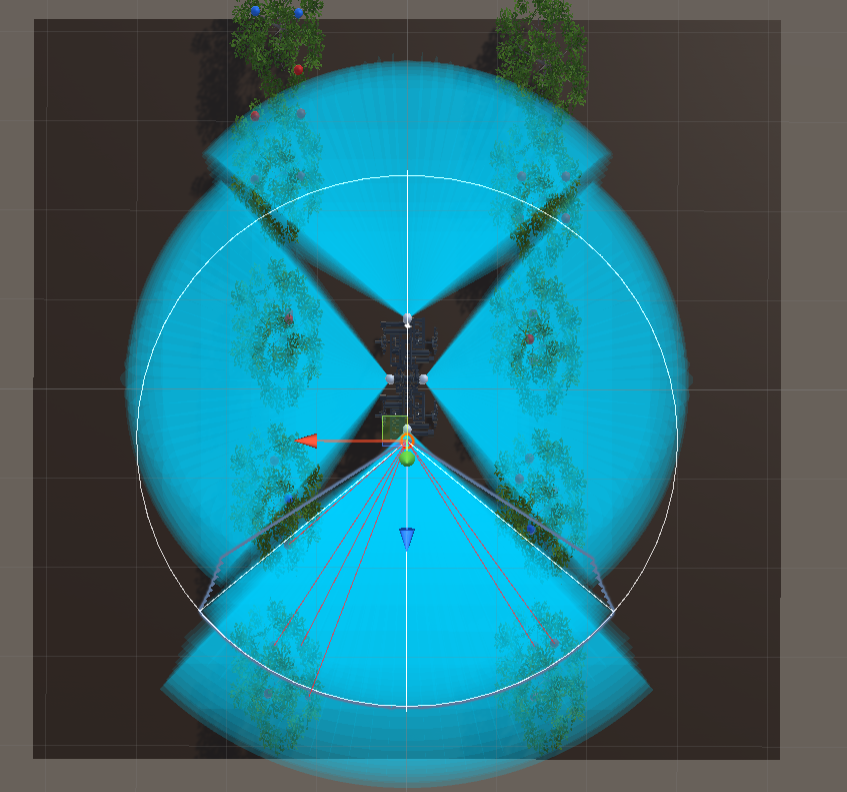
\includegraphics[width=0.8\linewidth]{FOV(29).png}
   \caption{Top view of Lealaps with 4x ZED2 depth Cameras and a Velarray M1600 Solid State Lidar at the front.}
\end{subfigure}
\begin{subfigure}[htbp]{1\textwidth}
   \centering
   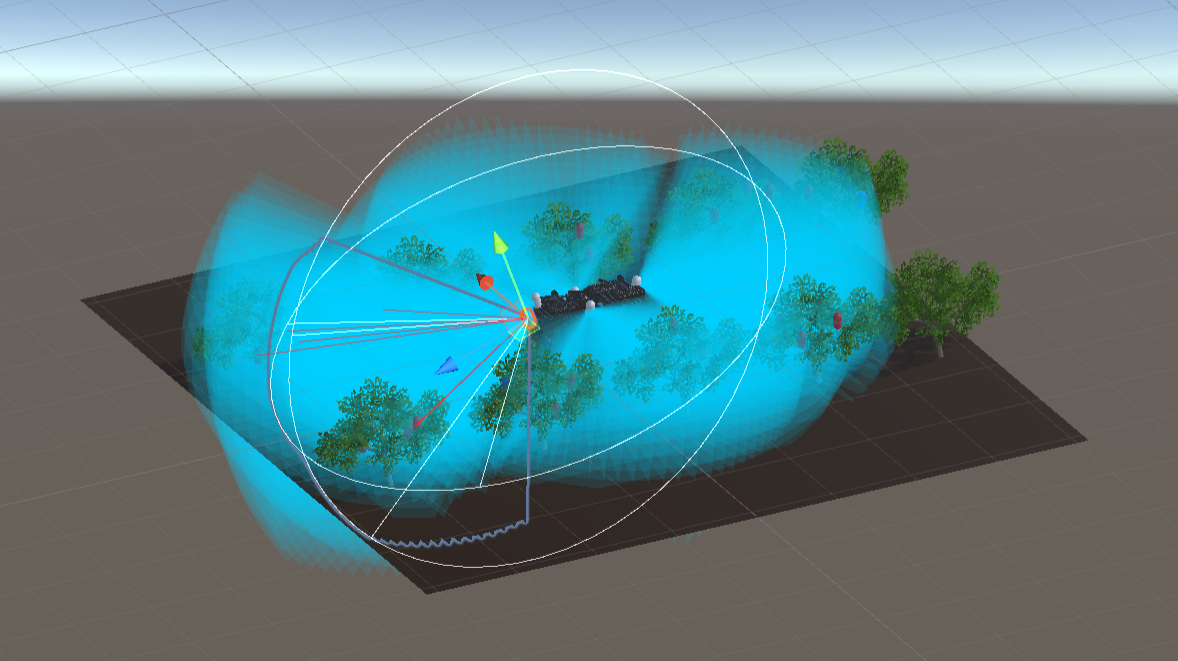
\includegraphics[width=0.8\linewidth]{FOV(30).png}
   \caption{Side view of Lealaps with 4x ZED2 depth Cameras and a Velarray M1600 Solid State Lidar at the front.}
\end{subfigure}
\caption[]{Using the FOV\_Visualizing tool in unity to check for blind spots and overall visibility constraints on the chosen sensor configuration for Laelaps.}
\end{figure}

\clearpage
\end{enumerate}
\printbibliography %Prints bibliography

\end{document}
  